\section{Пункты программы}

\section{1. Понятие временной и пространственной (по памяти) сложности алгоритма. Определение асимптотических сравнений $O, \Theta, \Omega$. Примеры.}
Временная и пространственная сложность алгоритма нужны для оценки и сравнения программ между собой. 

\Def Временная сложность - величина, характеризующая количество элементарных действий программы, то есть тех, которые работают условно за 1 такт работы процессора. 

Модель памяти(RAM-модель):
\begin{enumerate}
    \item Память вычислителя безгранична.
    \item Доступ к памяти на чтение/запись требует пренебрежимо малого времени(округляется единичкой)
\end{enumerate}

\Def Пространственная сложность - величина, характеризующая количество единиц доп.памяти, которые необходимы для выполнения программы.

\subsection*{Асимптотические сравнения}

\Def Пусть имеются две функции $f(n)$  и $g(n)$, при этом $f, g \; : \N \rightarrow \N$,
тогда считается, что $f(n) = \mathcal{O} (g(n))$, если $\exists C > 0 \; \ \exists N_{0}: \ \forall n > N_{0} \; \; f(n) \leqslant C \cdot g(n)$

\Def Пусть имеются две функции $f(n)$  и $g(n)$, при этом $f, g \; : \N \rightarrow \N$,
тогда считается, что $f(n) = \Omega (g(n))$, если $\exists C > 0 \; \ \exists N_{0}: \ \forall n > N_{0} \; \; f(n) \geqslant C \cdot g(n)$

\Def Пусть имеются две функции $f(n)$  и $g(n)$, при этом $f, g \; : \N \rightarrow \N$,
тогда считается, что $f(n) = \Theta (g(n))$, если $\exists C_{1}, C_{2} > 0 \; \ \exists N_{0}: \ \forall n > N_{0} \; \; C_{1} \cdot g(n) \leqslant f(n) \leqslant C_{2} \cdot g(n)$

\subsection*{Мастер-теорема}

\Thbd Пусть имеется рекуррента:

$$\begin{cases}
aT(\frac{n}{b}) + O(n^c)\text{,} & n > 1\\
O(1), & n = 1
\end{cases}$$\\
где $a \in \N,\,b \in \R,\,b > 1,\,c \in \R^{+}$
Тогда:
\begin{itemize}
    \item Если $c > log_b\,a$, то $T(n) = O(n^c)$
    \item Если $c = log_b\,a$, то $T(n) = O(n^c\,log\,n)$
    \item Если $c < log_b\,a$, то $T(n) = O(n ^ {log_b\,a})$
\end{itemize}

\pagebreak

\section{2. Бинарный поиск. Бинарный поиск по ответу. Временная сложность}
\subsection*{Бинарный поиск}
\Task Дан отсортированный массив A[1 : n]. Надо проверить, есть ли в нем элемент X. 

\Alg
Обозначим за $l = 1$ и $r = n$ левую и правую границы
рассматриваемого подмассива.
\begin{enumerate}
    \item Если диапазон валиден, то проверим, $ A[ \left\lfloor \frac{l+r}{2} \right\rfloor] \geq X$. 
    Иначе вернем границу.
    \item Если полученный результат истинен, то запускаем рекурсивно
поиск в левой половине массива.
    \item Иначе — в правой половине массива.
\end{enumerate}

\textit{Асимптотика.}
\begin{enumerate}
    \item Сравнивает средний элемент с X за O(1).
    \item Решает, продолжать в левой или правой половине за O(1).
    \item Запускается рекурсивно, уменьшая область поиска в два раза.
\end{enumerate}
Результат будет получен, когда длина диапазона (далее n) станет
равной 1. 
А значит всего шагов $\log_2 n$
$$O(log_2\,n) = O(log\,n)$$

$T(N) = T(n/2) + O(1)$. По Мастер-теореме $T(N) = O(log\,n)$

\subsection*{Бинарный поиск по ответу}
Пусть имеется монотонный предикат \( P(n) \), то есть
$$
\exists N_0 : 
\begin{cases}
P(n) = 0, & n < N_0 \\
P(n) = 1, & n \geq N_0
\end{cases}
$$

И перед нами стоит задача отыскать это \( N_0 \). Например, задача проверки наличия элемента \( X \) в отсортированном массиве. В данном случае предикат будет звучать как 

$$P(i) = 1 \iff a[i] \geq X.$$


\Alg
Пусть \( N_0 \) заведомо лежит в каком-то диапазоне \([l, r]\). Тогда алгоритм следующий:
\begin{enumerate}
    \item Если диапазон валиден, то вычислим \( P\left( \left\lfloor \frac{l+r}{2} \right\rfloor \right) \). Иначе вернем границу.
    \item Если полученный результат истинен, то \( N_0 \in [l, \left\lfloor \frac{l+r}{2} \right\rfloor] \). Запускаем рекурсивно поиск в левой половине массива.
    \item Иначе \( N_0 \in \left[\left\lfloor \frac{l+r}{2} \right\rfloor, r\right] \). Запускаем рекурсивно поиск в правой половине массива.
\end{enumerate}
\textit{Асимптотика.} \( O(\log n) \).
\pagebreak

\section{3. Вещественнозначный бинарный поиск (по ответу). Временная сложность.}
\Task

Пусть нам задана монотонная функция $f(x)$
и какое-то значение $C$ этой функции. Необходимо найти значение аргумента $x$ этой функции, такое, что $f(x)\,=\,C$. 

\begin{figure}[h]
    \centering
    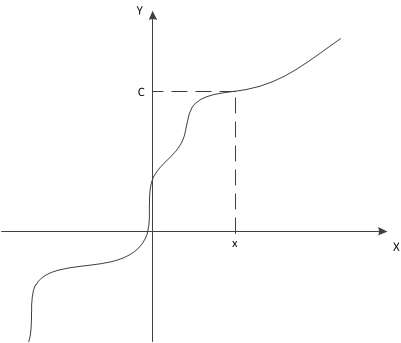
\includegraphics[width=0.3\linewidth]{pix/binsearch.png}
\end{figure}

\subsection*{Алгоритм}

Применим идею двоичного поиска. Выберем такие границы, где значение функции точно больше и точно меньше заданного значения. Выберем значение в середине этого отрезка. Если оно меньше, чем заданное, то сместим левую границу в середину отрезка. В противном случае сместим правую границу.

Есть несколько способов закончить поиск. К примеру, когда концы отрезка различается менее, чем на заданную погрешность $\varepsilon$.

\textit{Асимптотика.} $O\left(\log\left(\frac{r - l}{\epsilon}\right)\right)$.\\
\Proof\\
Мы знаем, что асимптотика целочисленного бинарного поиска - это $O(log\,n)$, где $n$ - длина промежутка, на котором запускается поиск. По сути, длина - это кол-во точек, в которых может оказаться искомое значение. Давайте узнаем "длину" для вещественного поиска. Искомая точка может оказаться в промежутках:
$\{[l, l + \epsilon), [l + \epsilon, l + 2\epsilon), \ldots\}$, то есть таких точек $\frac{r - l}{\epsilon}$ (Так как $\epsilon$ - это длина одного отрезка). А значит асимптотика вещественного бинарного поиска - $O\brackets{\log \brackets{\frac{r - l}{\epsilon}}}$. \Endproof
% \textit{Асимптотика.} $O\left(\frac{\log(r - l)}{\varepsilon}\right)$

\textbf{Псевдокод}

\begin{lstlisting}
double BinSearch(C: double) {
  left = findLeftBoard(C)
  right = findRightBoard(C)
  while (right - left > eps) {
    mid = (left + right) / 2
    if f(mid) < C {
      left = mid
    } else {
      right = mid
    }     
  }
  return (left + right) / 2
}
\end{lstlisting}
Источник: \href{https://neerc.ifmo.ru/wiki/index.php?title=Вещественный_двоичный_поиск}{Вещественный двоичный поиск}

\pagebreak

\hypertarget{prefsum}{}
\section{4. Префиксные суммы. Обобщение на произвольную обратимую операцию}
\Def \textit{Префиксная сумма} по $j$ элементам - это сумма первых $j$ элементов массива. 

\Task Есть массив из $n$ элементов $a_1, \ldots, a_n$ и $q$ запросов вида $(l_1, r_i), ..., (l_q, r_q)$. Требуется для каждого запроса вывести $\sum\limits_{j = l_i}^{r_i}a_j = a_{l_i} + a_{l_i + 1} + ... + a_{r_i}$, где $i$ - номер запроса. 

\Alg Посчитаем префиксные суммы для любого $j$ от $0$ до $n$: $pref_j = a_1 + ... + a_j$. Для $j = 0: pref_0 = 0$, для $j > 0: pref_j = pref_{j-1} + a_j$. Ответ на запрос $(l_i, r_i):$ $\sum\limits_{j = l_i}^{r_i}a_j = pref_{r_i} - pref_{l_i - 1}$.

\textit{Асимптотика:} Подсчёт всех значений $pref_j$ (по порядку) займёт $O(n)$ времени, подсчёт ответа на все запросы: $O(q)$. Итоговая асимптотика $O(n + q)$. 

\textbf{Обобщение на произвольную обратимую операцию}

Подобный прием можно использовать не только для сложения, но и для других операций, являющихся обратимыми:
\begin{enumerate}
    \item побитовое исключающее «или» $\oplus$
    \item сложение по модулю
    \item умножение
\end{enumerate}

\textbf{Алгоритм для произвольной операции.}

Посчитаем префиксные значения для любого $j$ от $0$ до $n$: 

$$pref_j = \text{op}(a_1, a_2, \ldots, a_j).$$

Для $j = 0$: $pref_0 = \text{identity}$, где $\text{identity}$ — это нейтральный элемент для операции $\text{op}$ (например, $0$ для сложения, $1$ для умножения). Для $j > 0$: 

$$pref_j = \text{op}(pref_{j-1}, a_j).$$

Ответ на запрос $(l_i, r_i)$: 

$$\text{op}\left(pref_{r_i}, \text{inverse}(pref_{l_i - 1})\right),$$

где $\text{inverse}(x)$ — это функция, возвращающая обратное значение для операции $\text{op}$ (например, $-x$ для сложения, $\frac{1}{x}$ для умножения).

\pagebreak

\section{5. Факторизация числа. Функция Эйлера. Сводимость вычисления функции Эйлера к факторизации.}
\section*{Факторизация.}

\Def Факторизация - процесс разложения числа делители.

\begin{enumerate}
    \item Линейный алгоритм. Для каждого i от 1 до n проверяем, что число n делиться на i.
\begin{lstlisting}
for (int i = 1; i <= n; ++i) {
  if (n % i == 0) {  
    cout << i << " ";  
  }  
}
\end{lstlisting}
    \item Если $d$ - делитель $n$, то и $n/d$ - делитель, а значит достаточно перебирать не до $n$, а до $[\sqrt{n}]$.
\begin{lstlisting}
for (int i = 1; i <= sqrt(n); ++i) {  
  if (n % i == 0) {  
    cout << i << " ";  
    if (i != n / i) {  
      cout << n / i << " ";  
    }  
  }  
}
\end{lstlisting}
\end{enumerate}

\textbf{Алгоритм разложения числа на простые делители (Оптимизированный).}

\begin{lstlisting}
int d = 2;
while (n > 1) {
  if (n % d == 0) {
    cout << d << " ";
    n /= d;
  } else if (d * d > n) {
    cout << n;
    break;
  } else {
    ++d;
  }
}
\end{lstlisting}

Написан на основе: \href{https://neerc.ifmo.ru/wiki/index.php?title=Разложение_на_множители_(факторизация)#.D0.9F.D1.81.D0.B5.D0.B2.D0.B4.D0.BE.D0.BA.D0.BE.D0.B4_.D0.BD.D0.B0.D1.85.D0.BE.D0.B6.D0.B4.D0.B5.D0.BD.D0.B8.D1.8F_.D0.BF.D1.80.D0.BE.D1.81.D1.82.D1.8B.D1.85_.D0.BC.D0.BD.D0.BE.D0.B6.D0.B8.D1.82.D0.B5.D0.BB.D0.B5.D0.B9}{Викиконспекты (ИТМО). Псевдокод нахождения простых делителей.}

\section*{Функция Эйлера.}

\Def Функция Эйлера от числа $n, \varphi(n)$, равна количеству чисел, меньших $n$ и взаимно простых с ним. 

Например, $\varphi(5) = 4$ (числа $1, 2, 3, 4$).

\textbf{Свойства функции Эйлера.}

\begin{enumerate}
    \item Если $p$ - простое, то $\varphi(p) = p - 1$.
    \item Если $p$ - простое, то $\varphi(p^\alpha) = p^\alpha - p^{\alpha - 1}$.
    \item Если $n, m$ взаимно просты, то $\varphi(m \cdot n) = \varphi(m) \cdot \varphi(n)$. 
\end{enumerate}

\textbf{Сводимость вычисления функции Эйлера к факторизации.}

Наивный алгоритм. Для каждого числа от 1 до $n$ проверяем, является ли делителем $n$.

Немного преобразований:

$$\varphi \brackets{n} = \varphi \brackets{\prod_{i}{p_{i}^{\alpha_i}}} = \prod_{i}\varphi\brackets{p^{\alpha_i}_{i}} = \prod_{i}\brackets{p^{\alpha_i}_{i} - p^{\alpha_i - 1}_{i}} = $$

$$\prod_{i}\brackets{p^{\alpha_i}_{i}\brackets{1 - \frac{1}{p_i}}}=\prod_{i}p^{\alpha_i}_{i} \cdot \prod_i\brackets{1 - \frac{1}{p_i}} = n \cdot \prod_i\brackets{1 - \frac{1}{p_i}}$$

Таким образом, зная факторизацию числа, можно вычислить $\varphi(n)$ за $\mathcal{O}(\log n)$.

\pagebreak

\section{6. Классическое решето Эратосфена за $O(n\,log\,log\,n)$ (время работы б/д). Линейное решето Эратосфена.}
\Def Решето Эратосфена - алгоритм, позволяющий найти все простые числа от 2 до n.

\section*{Решето Эратосфена}

\Alg 
\begin{enumerate}
    \item Берем минимальное непросмотренное число k, объявляем его простым.
    \item Далее все числа от 2 до n, кратные k объявляются непростыми.
    \item Повторить пока все числа не рассмотрены.
\end{enumerate}

\begin{lstlisting}
vector <bool> primes(n, true);  
primes[0] = primes[1] = false;
for (int i = 2; i < n; ++i) {
  if (!primes[i]) {
    continue;
  }
  for (int j = 2; i * j < n; ++j) {  
    primes[i * j] = false;  
  }
}
\end{lstlisting}

\textbf{Оптимизация.}
\begin{enumerate}
    \item Можно увеличивать $i$ на 2 каждый раз, так как кроме двойки все простые нечетные.
    \item Можно начинать перебирать $j$ начиная с $i$ , поскольку все числа меньшие $i^2$, кратные $i,$ обязательно имеют простой делитель меньше $i$, а значит, все они уже были отсеяны раньше.
\end{enumerate}

\textbf{Сложность решета Эратосфена.}


\Thbd Сложность алгоритма выше составляет $\mathcal{O}(n\log\log n)$, где $n$ - число, до которого ищем простые.

\section*{Линейное решето Эратосфена}

\Alg 
\begin{enumerate}
    \item Для каждого числа от 2 до n найдем минимальный простой делитель (массив mind). Тогда простые легко детектируются.
    \item При рассмотрении очередного числа i пройдемся по массиву уже найденных простых primes и будем обновлять минимальный делитель у просматриваемых чисел.
\end{enumerate}

\pagebreak

\begin{lstlisting}
vector<int> primes;
vector<int> mind(n + 1);

for (int i = 2; i <= n; ++i) {
  mind[i] = i;
}

for (int i = 2; i <= n; ++i) {
  if (mind[i] == i) {
    primes.push_back(i);
  }

  for (int p : primes) {
    if (p * i > n || p > mind[i]) {
      break;
    }
    mind[i * p] = p;
  }
}
\end{lstlisting}

\textbf{Сложность линейного решета Эратосфена.}

\begin{itemize}
    \item Внешний цикл for делает $O(n)$ операций: очевидно.
    \item Внутренний цикл также делает суммарно $O(n)$ операций: докажем.

    \Proof\\
    \textbf{Лемма 1}: $\forall n \in \mathbb{N}\;\; \exists!$ разложение $n = a \cdot b$, где $a$ - наименьший простой делитель $n$, а $b$ - остальная часть. Единственность очевидна из основной теоремы арифметики.\\
    \textbf{Лемма 2}: Каждая пара $(a, b)$, где $a$ - простое число, $b$ - натуральное число с наименьшим простым делителем $ > a$, делает ровно 1 изменение в массиве mind. Это следует из Леммы 1 (Каждая пара "бьёт"\ ровно в 1-у ячейку mind).\\
    \textbf{Лемма 3}: У нас не "сгенерируется"\ $> 1$ одинаковой пары $(a, b)$, то есть не будет такой ситуации, что $\exists a, b, c, d: (a, b), (c, d) \text{ и при этом } a \cdot b = c \cdot d$\\
    По итогу, так как у нас "генерируются"\ различные пары (a, b), каждая из которых обновляет ровно одну ячейку mind, то таких пар O(n) (Ведь mind.size() = O(n)), а значит вложенный массив суммарно делает O(n) операций.\\
    \Endproof
\end{itemize}

% Сложность определяется суммарным числом итераций внутреннего for.

% На первый взгляд для каждого p в разложении k изменяется mind[k]. Однако каждое mind[k] рассматривается ровно 1 раз, следовательно сложность линейная.

\pagebreak

\section{7. Арифметика в $Z_m$. Малая теорема Ферма и теорема Эйлера б/д. Критерий существования обратного по модулю. Поиск обратного по модулю.}
\Def Кольцо -- набор из множества «чисел» и операций сложения и
умножения, для которых верны все классические свойства этих
операций: ассоциативность, коммутативность,
дистрибутивность\dots Однако нет обратимости по умножению (нельзя
делить).

\Def Кольцо $\Z_m$ -- структура над числами $0, 1, \dots , m - 1$, где все
операции ведутся по модулю $m$

\Note Это наивное определение, которое в общем некорректно, но дает понимание того, с чем мы работаем.

\Def Отрицательное число в $\Z_m$: \space
$-b\,=\,
\begin{cases}
0,\:b\:=\:0\\
m - b,\:\text{иначе}
\end{cases}$

\Def $a^{-1} = b$ в $\Z_m$ тогда и только тогда, когда $a\,\cdot\,b\,\equiv\,1\,(mod \,m)$.

\Def Поле — набор из множества «чисел» и операций сложения и умножения, для которых верны все классические свойства этих операций: ассоциативность, коммутативность, дистрибутивность и обратимость.

\Note Это наивное определение, которое в общем некорректно, но дает понимание того, с чем мы работаем.

\Thbd (Малая теорема Ферма). Пусть $m$ -- простое, тогда
$1 = a^{m - 1}$ в $\Z_m$.

\Consequence Если $p$ -- простое, то $\Z_p$ -- поле, обратное тоже верно. То
есть для каждого ненулевого $a \in \Z_p$ существует $a^{-1}$

\Thbd  (Эйлер) Пусть $m \in \N$. Тогда для $a \in \Z_m$ существует  $a^{-1}$ тогда и только тогда, когда $gcd(a, m) = 1$. Более того, если $gcd(a,\,m)\,=\,1$, то $a^{-1} = a^{\varphi(m)-1}$ в $\Z_m$.


\pagebreak

\section{8. Критерий существования обратного по модулю. Поиск обратного по модулю. Алгоритм Евклида (классический и расширенный).}
\subsection*{Алгоритм Евклида}

\begin{lstlisting}
int gcd(int a, int b) {
    while (b != 0) {
        a %= b;
        swap(a, b);
    }
    return a;
}
\end{lstlisting}

\subsection*{Расширенный алгоритм  Евклида}

Расширенный алгоритм находит, помимо $g = gcd(a,\,b)$,  такие целые коэффициенты x и y, что $a \cdot x + b \cdot y = g$
Пусть мы посчитали нужные коэффициенты $x'\,\text{и}\,y'$, когда рекурсивно считали $gcd(b,\,a\,mod\,b)$. Иными словами, у нас есть решение $(x',\,y')$ для пары $(b,\,a\,mod\,b)$

$$b \cdot x' + (a\,mod\,b) \cdot y' = g$$

Чтобы получить решение для исходной пары, запишем выражение $(a\,mod\,b)$ по определению как $(a - \lfloor{\frac{a}{b}}\rfloor \cdot b)$ и подставим в приведенное выше равенство

$$b \cdot x' + (a - \lfloor{\frac{a}{b}}\rfloor \cdot b) \cdot y' = g$$

Теперь выполним перегруппировку слагаемых (сгруппируем по исходным a и b) и получим:

$$a \cdot y' + b \cdot (x' - \lfloor{\frac{a}{b}}\rfloor \cdot y') = g$$


$$\begin{cases}
x = y'\\
y = x' - \lfloor{\frac{a}{b}}\rfloor \cdot y'
\end{cases}$$

\begin{lstlisting}
int gcd(int a, int b, int &x, int &y) {
  if (b == 0) {
    x = 1;
    y = 0;
    return a;
  }
  int x1, y1;
  int d = gcd(b, a % b, x1, y1);
  x = y1;
  y = x1 - (a / b) * y1;
  return d;
}
\end{lstlisting}

Рассмотрим уравнение $ax + my = 1$. Возьмем обе части по модулю m
и $ax = 1 \Rightarrow x = a^{-1}$

То есть с помощью расширенного алгоритма Евклида ищем обратный
элемент в $\Z_m\,\text{за}\,O(log\,m)$.

Стоит отметить, что расширенный алгоритм Евклида не гарантирует, что $x < m$, поэтому нужно будет дополнительно сделать $x = x\; \%\; m$.

\pagebreak

\section{9. Амортизированный анализ. Метод монеток. Применение на примере push\_back в динамическом массиве}
\Def Пусть имеется последовательность операций, каждая из которых
выполняется за время $t_i$ , тогда амортизированная стоимость операции {\large $t^* = \frac{1}{n} \sum\limits_{i=1}^n t_i$}

\begin{center}
Метод монеток
\end{center}

\begin{enumerate}
    \item Допустим, что каждая операция стоит определенной количество
монет $C_i$ — учетная стоимость.
    \item Учетная стоимость не менее реальной. Тогда резерв уйдет на
покрытие остальных операций.
\end{enumerate}

Пример. Динамически расширяющийся массив
\begin{enumerate}
    \item Пусть каждый push, не требующий перевыделения памяти стоит 3 монетки. Одна монетка на запись элемента и две монетки в резерве (будем их класть на элементы массива с номерами $i$ и $i\,-\,\frac{n}{2}$ ).
    \item Инвариант. Перед каждой реаллокацией на каждом элементе есть по монете.
    \item Этими монетами оплачиваем перекопирование.
    \item То есть амортизированная сложность push равна $O(1)$.
\end{enumerate}

\pagebreak

\section{10. Амортизированный анализ. Метод потенциалов. Применение на примере push\_back в динамическом массиве.}
\Def. Потенциалом от структуры S назовем такую функцию $\varphi(S)$, что:
\begin{enumerate}
    \item $\varphi(S_0) = 0$, где $S_0$ — изначальное состояние структуры
    \item $\varphi(S) \geq 0$ в любой момент времени.
\end{enumerate}

\Def Пусть $t_i$ — реальное время i-й операции, тогда
$t^*_i = t_i + \varphi(S_i) - \varphi(S_{i-1})$ — учетное время.

\Statement $\frac{1}{n} \sum\limits_{i=1}^n t_i^* \geq t^*$

\begin{center}
Пример. Динамически расширяющийся массив
\end{center}

Пусть c — вместимость массива, а s — его размер.
Введем $\varphi(S) = 2s - c$. Так как реаллокация в два раза, все требования
выполняются. Посчитаем $t_i^*$.

\begin{enumerate}
    \item Реаллокация не нужна $\varphi(S_i) - \varphi(S_{i-1}) = 2$, то есть $t_i^* = 3$
    \item Реаллокация нужна, то есть (s, c) $\rightarrow$ (s + 1, 2c) и c = s.
\end{enumerate}

$$\varphi(S_i) - \varphi(S_{i-1})\,=\,2(s\,+\,1)\,-\,2s\,-\,(2s\,-\,s)\,=\,2\,-\,s$$

Откуда $t_i^* = s + 2 - s = 2$

\pagebreak

\section{11. Линейные контейнеры. Односвязный и двусвязный списки. Стек, очередь, дек (через списки и
через кольцевой буффер).}
\Def Контейнер — некоторая структура, позволяющая хранить
некоторые данные. Например, массив.

\Def Контейнер линейный, если на нем однозначно определено
отношение «следующий элемент».

\Def Список — последовательный набор узлов, предоставляющий
следующий интерфейс.

\begin{center}
   \centering
   \begin{tabular}{|c|c|c|}
    \hline
    Операция                        & Время & Примечание          \\ \hline
    Вставка в начало                & O(1)  &                     \\ \hline
    Удаление из начала              & O(1)  &                     \\ \hline
    Вставка в конец                 & O(1)  & Если двусвязный     \\ \hline
    Удаление из конца               & O(1)  & Если двусвязный     \\ \hline
    Вставка в произвольное место    & O(1)  & Если известно место \\ \hline
    Удаление из произвольного места & O(1)  & Если известно место \\ \hline
    Поиск                           & O(N)  &                     \\ \hline
    Обращение по индексу            & O(N)  &                     \\ \hline
    \end{tabular}
\end{center}

\Def Односвязный список -- последовательный набор из узлов с
данными, где каждый узел знает, где лежит следующий за ним.

\Def Двусвязный список -- последовательный набор из узлов с
данными, где каждый узел знает, где лежат следующий и предыдущий
узлы.

\Def Стек stack -- структура данных, которая хранит элементы и
предоставляет к ним доступ в рамках парадигмы LIFO (Last in, First
Out).
Можно реализовать на массиве и на односвязном списке.

\Def Очередь queue -- структура данных, которая хранит элементы и
предоставляет к ним доступ в рамках парадигмы FIFO (First in, First
Out).
Можно реализовать на двусвязном списке.

\Def Дек deque -- структура, представляющая из себя двустороннюю
очередь, то есть можно вставлять/удалять в начало/конец.
Можно реализовать на двусвязном списке.

\begin{center}
Стек с минимумом
\end{center}

При добавлении нового элемента в стек $S$ для получения стека $S'$
будем в голову $S'$ добавлять минимум как минимум из значения
элемента и значения минимума в голове $S'$.

\begin{center}
Очередь на двух стеках
\end{center}

Сделаем один стек на вход stack\_in и второй на выход stack\_out. В
первый будем добавлять, а из второго — извлекать.
Если при извлечении stack\_out пуст, то перекидываем все элементы
из stack\_in в stack\_out.

\begin{center}
Очередь c поддержкой операции получения минимума
\end{center}
Заведем очередь на двух стеках, поддерживающих минимум.
Запрос минимума сводится к минимуму из минимумов в двух стеках.

\pagebreak

\section{12. Линейные контейнеры. Очередь с поддержкой произвольной ассоциативной операции.}
\Def Операция $f$ ассоциативна, если $f (a, f (b, c)) = f (f (a, b), c)$.

\Def Операция $f$ коммутативна, если $f (a, b) = f (b, a)$.

Сначала реализуем стек с поддержкой произвольной ассоциативной операции. Для этого стек должен хранить пары. Для наглядности рассмотрим пример абстрактного стека, который хранит нужные пары вида $\{a, b\}$, где $a$ - непосредственно сам элемент, $b$ - значение функция от $a$ и элементов "ниже"\ $a$ (Индекс обозначает порядок добавления в стек):

\begin{table}[h]
\centering
\begin{tabular}{|l|l|}
\hline
$el_4$ & $f(el_4, f(el_3, f(el_2, el_1)$  \\
\hline
$el_3$ & $f(el_3, f(el_2, el_1)$           \\
\hline
$el_2$ & $f(el_2, el_1)$                    \\
\hline
$el_1$ & $el_1$\\
\hline
\end{tabular}
\end{table}

Реализация поддерживания подобной структуры при классическом добавлении/удалении элемента из стека очевидна.
\vspace{1cm}


Перейдём от стека к очереди.

Для этого будем поддерживать 2 стека с подобной структурой: стека на вход stack\_in, стек на выход stack\_out. В
первый будем добавлять, а из второго — извлекать.
Если при извлечении stack\_out пуст, то перекидываем все элементы
из stack\_in в stack\_out. Разумеется, мы поддерживаем вышеуказанную структуру в обоих стеках после каждого их удалений/добавлений.\\
Чтобы узнать $f$ от всех элементов очереди, достаточно получить значение $f(b_1, b_2)$, где $b_1, b_2$ - 2-ые элементы "верхних"\ пар стеков stack\_in и stack\_out.

\pagebreak

\section{13. Сортировки. Теорема о нижней границе времени сортировки. Стабильные сортировки.}
\Def Сортировка набора элементов $a_1, \dots , a_n$ — задача поиска такой
перестановки индексов $\sigma$, что {\large $a_{\sigma(1)} \leq a_{\sigma(2)} \leq \, \dots \, \leq a_{\sigma(n)}$}.

\Lemma $\log{n!}=\Theta(n\log{n})$\\
\Proof
$$\log{n!}=\log{1}+\log{2}+\ldots+\log{n} \leq n\log{n} \Rightarrow \log{n!}=O(n\log{n})$$
$$\log{n!} \geq \frac{n}{2}\cdot \log{\frac{n}{2}} = \frac{n}{2}(\log{n} - \log{2}) = \frac{1}{2}n\log{n} - \frac{1}{2}n\log{2} \Rightarrow \log{n!}=\Omega(n\log{n})$$
Следовательно, $\log{n!}=\Theta(n\log{n})$ \Endproof

\Th Сортировка N элементов, основанная на сравнениях, требует $\Omega(N\,log\,N)$ сравнений.

\Proof \\ Задача состоит в поиске одной из $n!$ перестановок. Заметим, что при ответе на запрос: какое из двух чисел должно стоять раньше? - количество перестановок уменьшается в два раза. То есть $n! \mapsto \frac{n!}{2} \mapsto \frac{n!}{4} \mapsto \ldots \;$, что влечет хотя бы $\log{n!}$ итераций $\Rightarrow$ (по лемме) $\Omega(n\log{n})$. \Endproof

\Def Сортировка стабильная, если одинаковые с точки зрения компаратора элементы не меняют своего относительного расположения.

Из рассмотренных сортировок ранее, только MergeSort стабильная

\pagebreak

\section{14. Сортировка слиянием. Подсчет числа инверсий.}
\subsection*{Процедура Merge}

\Task Даны два отсортированных массива $a_1 \leq\,\dots\,\leq a_n$ и
$b_1 \leq\,\dots\,\leq b_m$. Надо слить их в один отсортированный за O(n + m)
времени и доппамяти.

\Solve 
\begin{enumerate}
    \item Заведем указатели на первые элементы массивов i и j.
    \item По индексу i + j выпишем меньший из $a_i$ и $b_j$ и сдвинем соответствующий указатель на один вперед.
    \item Так делаем, пока i < n \&\& j < m.
    \item Оставшийся хвост одного из массивов дописываем в конец.
\end{enumerate}

\subsection*{MergeSort}

\Task Дан массив $a_1, \dots , a_n$. Необходимо отсортировать его за
$O(n\,log\,n)$ времени и $O(n)$ доппамяти

\Solve
\begin{enumerate}
    \item Разделим массив на две равные части.
    \item Каждую из них рекурсивно отсортируем.
    \item Результаты сольем в один отсортированный массив с помощью процедуры Merge.
\end{enumerate}

\subsection*{Инверсии}

\Def Пара i < j называется инверсией, если $a_i > a_j$.

\Task Дан массив $a_1, \dots , a_n$. Необходимо найти число инверсий за
$O(n\,log\,n)$ времени и $O(n)$ доппамяти.

\Solve 
\begin{enumerate}
    \item Если при слиянии элемент левой части больше элемента правой части, то значит это и есть инверсия.
    \item Пусть мы сравниваем в сортировке слиянием l[i] и r[j], тогда если $r[j] < l[i]$, то $r[j] < l[i] < l[i + 1] <\, \dots \,< l[N]$, то есть число инверсий это N - i для r[j].
    \item Тогда для одного слияния итоговое число инверсий равно сумме по j таких значений.
    \item Итоговый ответ равен сумме по всем слияниям.
\end{enumerate}

\pagebreak

\section{15. Бинарная пирамида. Определение. Поддержка свойства пирамиды.}
\subsection*{Определение}

\Def Куча — структура данных, которая позволяет добавлять в себя
элементы и получать/извлекать минимум за логарифмическое время.

\Def Бинарная куча  — это такое бинарное дерево, для которого выполнены следующие три условия:
\begin{enumerate}
    \item Значение в любой вершине не больше (если куча для минимума), чем значения её потомков.
    \item На \(i\)-ом слое \(2^i\) вершин, кроме последнего.
    \item Последний слой заполнен слева направо.
\end{enumerate}

\subsection*{Поддержка свойства пирамиды}

\subsubsection*{Реализация кучи на массиве}

Удобнее всего двоичную кучу хранить в виде массива $tree[0..n-1]$, у которого нулевой элемент, $tree[0]$ — элемент в корне, а потомками элемента $tree[i]$ являются $tree[2i+1]$ и $tree[2i+2]$.

\begin{figure}[h!]
        \centering
        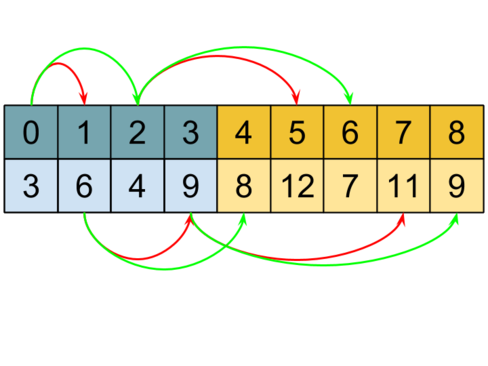
\includegraphics[scale=0.45]{pix/heap_on_an_array.png}
        \caption {Красная стрелка - левый сын, зеленая - правый сын}
        \label{fig:first}
\end{figure}

\subsubsection*{SiftDown}

\Def Просеивание элемента вниз — процедура, погружающая элемент
как можно ниже, пока не выполняется свойство кучи.

\begin{lstlisting}
void Heap::SiftDown(int i) {
  while (2 * i + 1 < size) {
    leftChildIndex = 2 * i + 1;
    rightChildIndex = 2 * i + 2;
    minIndex = i;

    if (tree[leftChildIndex] < tree[minIndex]) {
      minIndex = leftChildIndex;
    }
      
    if (rightChildIndex < size && tree[rightChildIndex] < tree[minIndex]) {
      minIndex = rightChildIndex;
    }

    if (minIndex == i) break;

    swap(tree[i], tree[minIndex]);
    i = minIndex;
  }
}
\end{lstlisting}

\Correctness SiftDown:

Пусть в дереве выполняются все неравенства между детьми и родителями, кроме, может быть, одного элемента $tree_i$, для которого $tree_i$ > $tree_{2i + 1}$ и (или) $tree_i$ > $tree_{2i+2}$. Тогда после выполнения операции SiftDown корректность восстановится.

\drawsome{pix/heap_sift_down.png}

Рассмотрим 5 случаев взаимного соотношения элементов $tree_{i}$ ,$tree_{2i+1}$, $tree_{2i+2}$.
\begin{itemize}
    \item $tree_{i} \leq tree_{2i + 1}$ и $tree_{i} \leq tree_{2i+2}$. Тогда мы заходим в цикл, но ни в первое, ни во второе условие не попадаем, minIndex остается равным i, и мы выходим из функции. Дерево корректно.

    \item $tree_{i}$ > $tree_{2i + 1}$ и $tree_{i} \leq tree_{2i+2}$. Тогда мы заходим в цикл, а после в первое условие. minIndex = leftChildIndex. Во второе условие мы не заходим, в третье тоже. Меняем местами левого ребенка и родителя. Тогда новый родитель больше обоих детей. Тут все корректно. Т.к. оба поддерева изначально были корректны, то мы могли что-то нарушить только в левом поддереве. Идем туда.
     \item $tree_{i} \leq tree_{2i + 1}$ и $tree_{i}$ > $tree_{2i+2}$. Рассуждения аналогичны расссуждению в п.2.
     \item $tree_{i}$ > $tree_{2i + 1}$ и $tree_{i}$ > $tree_{2i+2}$. Тут мы заходим в цикл, а после сразу попадаем в первое условие. minIndex = leftChildIndex.
     Если правый ребенок меньше левого, то он будет новым родителем, т.к. в этом случае правый ребенок является минимальным элементном из трех. Иначе - левый ребенок минимальный. И он станет новым родителем. Меняем родителя с минимальным из детей и идем дальше, нужно проверить, не нарушили  ли мы что-то в ветке, в которой был минимальный ребенок.
    
    \item Если детей нет, в цикл не заходим, все корректно, функция завершает работу. Если есть только один ребенок, то сравнение происходит только с ним. \Endproof
\end{itemize} 

\subsubsection*{SiftUp}

\Def Просеивание элемента вверх — процедура, поднимающая элемент
как можно выше, пока не выполняется свойство кучи.

\begin{lstlisting}
void Heap::SiftUp(int i) {
  int parentIndex = (i - 1) / 2;
  while (i > 0 && tree[i] < tree[parentIndex]) {
    swap(tree[i], tree[parentIndex]);
    i = parentIndex;
    parentIndex = (i - 1) / 2;
  }
}
\end{lstlisting}

\Correctness SiftUp:

Пусть в дереве выполняются все неравенства между детьми и родителями, кроме, может быть, одного элемента $tree_i$, для которого  $tree_i$ < $tree_{(i-1)/2}$ Тогда после выполнения операции SiftUp корректность восстановится.

\drawsome{pix/heap_sift_up.png}

Рассмотрим 2 случая:
\begin{itemize}
    \item Если элемент корневой или $tree_{i} \geq tree_{(i-1)/2}$ тогда дерево корректно, и в цикл мы не заходим, функция завершает выполнение.
    \item Если $tree_{i}$ < $tree_{(i-1)/2}$, то меняем местами родителя и ребенка. Новый родитель не увеличивается, поэтому неравенства между новым родителем и другим ребенком остаются корректными, при этом восстанавливаются неравенства между родителем и двумя детьми. В поддеревьях все ок. Но могло что-то нарушиться выше, поэтому текущий родитель становится ребенком, и процесс повторяется. \Endproof
\end{itemize} 

Выполняя операции SiftUp() и SiftDown() мы переходим между уровнями, на каждом из которых выполняем C = const количество операций. Высота дерева - $log(n)$, поэтому каждая из операций выполняется за время, не превосходящее $C \cdot log(n)$. Таким образом асимптотика $O(log(n))$.

\pagebreak

\section{16. Бинарная пирамида. Определение. Основные операции.}
\subsection*{Основные операции:}

\textbf{Insert: }
 \begin{lstlisting}
void Heap::Insert(int x) {
  tree.push_back(x); 
  ++size; 
  SiftUp(size - 1); 
}
\end{lstlisting}
Вставляем элемент в конец. Тогда могли нарушиться только неравенства с родителем. Поэтому необходимо просеять наверх.
\textit{Асимптотика: O(log(n)) за счет выполнения операции SiftUp()}

\textbf{GetMin: }
 \begin{lstlisting}
int Heap::GetMin() { 
  return tree[0]; 
}
\end{lstlisting}
Минимальный элемент кучи лежит в вершине дерева, просто его выводим. 
\textit{Асимптотика: O(1)}

\textbf{ExtractMin: }
 \begin{lstlisting}
void Heap::ExtractMin() {
  tree[0] = tree[size - 1]; 
  tree.pop_back();
  --size;
  SiftDown(0);
}
\end{lstlisting}
Меняем первый элемент и последний местами, удаляем последний. Т.к. у первого элемента нет родителей, то неравенства могли нарушиться только с детьми, поэтому просеиваем элемент вниз.\\
\textit{ Асимптотика: O(log(n)) за счет выполнения операции SiftDown()}

\pagebreak

\section{17. Бинарная пирамида. Определение. Операция Heapify (время работы O(n) б/д). Пирамидальная сортировка.}
\subsection*{Операция Heapify}

\Def Heapify -- процесс построения кучи на заданном массиве. То есть
надо переупорядочить элементы в массиве так, чтобы по индексам на
всех парах родитель-сын было соблюдено свойство кучи.

\Solve Будем просеивать вниз элементы, начиная с $\frac{N}{2}$-го и до
нулевого.

\Proof 
Элементы с индексами больше $\frac{N}{2}$ не могут быть родителями в куче, значит изначально для них правило кучи не нарушается.
До вызова SiftDown для вершины, ее поддеревья являются кучами.
После выполнения SiftDown эта вершина с ее поддеревьями будут также являться кучей. 
Значит, после выполнения всех SiftDown получится куча. 
\Endproof

\Th Время работы данного алгоримта: O(n).

\Proof \\
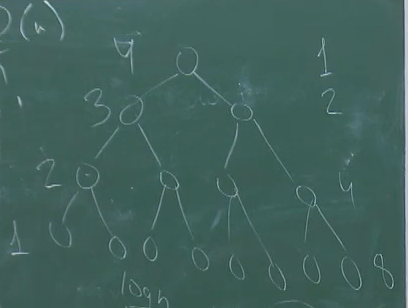
\includegraphics[width=5cm]{pix/25.png}

$\displaystyle\sum_{h=1}^{\log_{2}{n}} h*2^{\log_{2}{n} - h}$ = $n*\displaystyle\sum_{h=1}^{\log_{2}{n}} \frac{h}{2^h}$
 
$\displaystyle\sum_{h=1}^{\log_{2}{n}} \frac{h}{2^h}$ сходится к 2. Таким образом $T(n) = 2n$. Асимптотика O(n).
\Endproof

\begin{lstlisting}
void Heap::heapify() {
  for (int i = size / 2 - 1; i >= 0; --i) {
    siftDown(i);
  }
}
\end{lstlisting}

\subsection*{Пирамидальная сортировка}

\Task Отсортировать массив $a_1, \dots , a_n$ за $O(n\,log\,n)$ времени и $O(1)$ доппамяти.

\Solve 
\begin{enumerate}
    \item Выполнить Heapify.
    \item Пусть x = GetMin(), далее надо сделать ExtractMin() и вместо последнего элемента выписать x.
    \item Повторить это действие n - 1 раз.
    \item Развернуть массив.
\end{enumerate}

\pagebreak

\section{18. Быстрая сортировка. Процедура Partition за $O(1)$ доппамяти. Оценка времени с случайным
пивотом (б/д).}
\subsection*{QuickSort}

\Alg 
\begin{enumerate}
    \item Выбрать опорный элемент pivot.
    \item Произвести процедуру Partition, то есть распределить элементы в следующем порядке \textbf{(*)}:
    \begin{enumerate}
        \item Элементы $<$ pivot. Положим, что они занимают отрезок $[i_1, i_2].$
        \item Элементы $=$ pivot. Положим, что они занимают отрезок $[i_2 + 1, i_3].$
        \item Элементы $>$ pivot. Положим, что они занимают отрезок $[i_3 + 1, i_4]$
    \end{enumerate}
    \item Вызвать рекурсивно от $[i_1, i_2]$ и $[i_3 + 1, i_4]$.
\end{enumerate}

\subsection*{Пример процедуры Partition}

(Нам дают индексы left, right - начало и конец сортируемого отрезка, pivot - опорный элемент, vec - сортируемый массив) 

\begin{enumerate}
    \item Распределим элементы так, чтобы сначала шли все элементы $<$ pivot, а потом - все остальные:\\
    
    У нас есть индексы r0 и i. Мы поддерживаем инвариант: vec[i] < vec[r0]. Мы также постепенно двигаем i вправо, а r0 влево. Если инвариант перестаёт поддерживаться, то мы меняем местами значения vec[i] и vec[r0].
    \item Теперь распределим элементы так, чтобы выполнялось \textbf{(*)}:\\

    У нас есть индексы l0 и i (Стоит отметить, что l0 изначально стоит в элементы, где vec[l0] $\geq$ pivot. Мы поддерживаем инвариант: vec[l0] < vec[i]. Мы также постепенно двигаем l0 вправо, а i влево. Если инвариант перестаёт поддерживаться, то мы меняем местами значения vec[l0] и vec[i].
\end{enumerate}

Теперь просто найдём индексы, где начинается/заканчивается отрезок из элементов $=$ pivot и вернём пару из таких индексов.

% \begin{lstlisting}
% pair<int, int> Partition(int[] array, int l, int r) {
%   int pivot = ChoosePivot(array, l, r);
%   int i = l, j = r;
%   while(i <= j) {
%     while (array[i] < pivot) { ++i; }
%     while (array[j] > pivot) { --j; }
%     if (i >= j) { break; }
%     Swap(array[i], array[j]); ++i; --j;
%   }
%   return {j, i};
% }
% \end{lstlisting}

\begin{lstlisting}
#include <vector>

std::pair<int, int> Partition(int left, int right, int pivot,
                              std::vector<int>& vec) {
  int r0 = right;
  while (r0 != left && vec[r0] >= pivot) {
    r0--;
  }
  for (int i = left; i < r0; ++i) {
    if (vec[i] >= pivot) {
      while (r0 > i && vec[r0] >= pivot) {
        r0--;
      }
      if (i < r0) {
        std::swap(vec[i], vec[r0]);
        r0--;
      }
    }
  }
  int l0 = left;
  while (vec[l0] < pivot) {
    l0++;
  }
  for (int i = right; i > l0; --i) {
    if (vec[i] == pivot) {
      while (l0 < i && vec[l0] == pivot) {
        l0++;
      }
      std::swap(vec[i], vec[l0]);
      l0++;
    }
  }
  int idx1 = left;
  while (vec[idx1] != pivot) {
    idx1++;
  }
  int idx2 = right;
  while (vec[idx2] != pivot) {
    idx2--;
  }
  return {idx1, idx2};
}
\end{lstlisting}

\Thbd Среднее время работы быстрой сортировки при случайном выборе pivot составит $O(N\,log\,N)$, а доппамять логарифмична.

\pagebreak

\section{19. Поиск порядковой статистики. Оценка времени с случайным пивотом (б/д).}
\Def k-я порядковая статистика массива -- такой элемент, что после
сортировки массива он окажется на k-м месте.

\subsection*{Рандомизированная версия}

\begin{enumerate}
    \item Выбрать опорный элемент
    \item Провести разбиение
    \item Если индекс опорного элемента i окажется больше данного k, то нам надо искать слева k-ю порядковую, в случае равенства завершаемся, в противном случае надо искать $(i - k - 1)$-ю порядковую
\end{enumerate}

\Thbd Время работы этого алгоритма при случайном выборе pivot в среднем линейно.

\pagebreak

\section{20. Алгоритм медианы медиан. Время поиска медианы медиан.}
\Def Медианой массива называют его $\frac{N}{2}$-ю порядковую статистику. Получается, оптимальнее всего брать медиану в качестве pivot.

Нам требуется описать алгоритм поиска медианы за линейное время, но мы будем решать более общую задачу поиска k-й порядковой статистики за линейное время, которая покрывает задачу поиска медианы

\Alg Поиск медианы медиан
\begin{enumerate}
\item Разбить массив на блоки по пять.
\item Отсортировать блоки (можно пузырьком).
\item Выбрать медианы блоков.
\item Для массива медиан найдем его медиану. Найденный элемент назовем медианой медиан.
\end{enumerate}

\subsection*{Детерминированный алгоритм поиска k-й порядковой статистики}

\Statement Медиана медиан гарантированно делит массив в соотношении не хуже чем 3 : 7.

\Proof Cначала определим нижнюю границу для количества элементов, превышающих по величине опорный элемент x. В общем случае как минимум половина медиан, найденных на втором шаге, больше или равны медианы медиан x.
\\Таким образом, как минимум $\frac{N}{10}$ групп содержат по 3 элемента, превышающих величину x, за исключением группы, в которой меньше 5 элементов и ещё одной группы, содержащей сам элемент x. Таким образом получаем, что количество элементов больших x не менее $\frac{3N}{10}$. \Endproof

\Alg
\begin{enumerate}
    \item Найдем медиану медиан массива.
    \item Возьмем ее в качестве pivot.
    \item Проведем Partition.
    \item Если индекс опорного элемента i окажется больше данного k, то нам надо искать слева k-ю порядковую, в случае равенства завершаемся, в противном случае надо искать (i - k - 1)-ю порядковую.
\end{enumerate}

\Statement Данный алгоритм работает в худшем случае за $O(N)$ времени.

\Proof У нас есть три составляющих работы алгоритма на каждом шаге:
\begin{enumerate}
    \item Время на разделение массива на пятерки и сортировка каждой из них: $cN$.
    \item Время на поиск медианы медиан $T(\frac{N}{5})$.
    \item Время на поиск k-й порядковой не превзойдет времени его поиска в большей доле, то есть $T(\frac{7N}{10})$.
\end{enumerate}

Таким образом $T(N)\,=\,T(\frac{N}{5})+\,T(\frac{7N}{10})\,+\,cN$

По индукции: $T(N) \leq 10cN$

Следовательно $T(N)\,=\,T(\frac{N}{5})+\,T(\frac{7N}{10})\,+\,cN \leq \frac{10cN}{5} +\frac{7 \cdot 10cN}{10}\,+\,cN\,=\,10cN$ $\Rightarrow O(N)$
\Endproof

\pagebreak

\section{21. Алгоритмы и время работы быстрой сортировки с использованием алгоритма медианы медиан.}
\subsection*{Детерминированная быстрая сортировка}

\Alg
\begin{enumerate}
    \item Найдем медиану через детерминированный алгоритм поиска k-й порядковой статистики.
    \item Проведем по ней Partition.
    \item Рекурсивно запустимся от каждой из частей.
\end{enumerate}

\Statement Время работы такой быстрой сортировки составит $O(N\,log\,N)$ в худшем случае.

\Proof \\
$T(n)\,=\,2T(\frac{n}{2})\,+\,O(n)$ где ($O(n)$ здесь поиск медианы + Partition). \\По Мастер-теореме $T(n)\,=\,O(n\,log\,n)$ \Endproof

\pagebreak

\section{22. Сортировка подсчетом. Стабильный вариант. Алгоритм LSD.}
\subsection*{Counting sort}

Пусть известно, что множество объектов, массив из которых нам придется сортировать, невелико по размеру.
Тогда можно посчитать, сколько раз встречается каждый элемент, а потом вывести его нужное число раз.
Пусть множество сортируемых элементов имеет размер K, тогда время равно $O(N + K)$ и доппамять $O(K)$

\subsection*{Stable counting sort}

Пусть имеется массив A длины N -- исходный и массив B -- куда будем писать ответ. Также заведем массив P размера K , где K -- размер множества элементов.

\begin{enumerate}
    \item Пройдем по массиву A и запишем в P[i] число объектов с ключом i.
    \item Посчитаем префиксные суммы массива P, тогда мы знаем, начиная с какого индекса массива B надо писать структуру с ключом i.
    \item Идем по массиву A и пишем в нужное место, поддерживая, куда писать следующий элемент с ключом k.
\end{enumerate}

\subsection*{Least Significant Digit (LSD)}

Алгоритм Least Significant Digit сортирует целые беззнаковые числа за
линейное время.
unsigned int хранятся в виде строки из четырех байтов.
Тогда будем сортировать побайтово данные числа как
двоичные строки, сначала сортируем по убыванию последнего байта,
потом стабильно по убыванию второго байта и так далее. Важно использовать стабильную сортировку (к примеру сортировку подсчетом). После такого
получим, что массив чисел отсортирован.
Работает это за $O(Nk)$ времени, где k это число байтов или 4, то есть
за $O(N)$.

\pagebreak

\section{23. Бинарное дерево поиска. Определение, операции Find, Insert, Erase.}
\subsection*{Определение}

\Def Бинарным деревом поиска называют бинарное дерево, в котором
в поддереве левее все элементы не больше элемента в данном узле, а
в поддереве правее — строго больше.

\drawsome{pix/binary_search_tree.svg.png}

\subsection*{Find}

\Alg

\begin{enumerate}
    \item Допустим, мы находимся в узле c элементом cur\_val, а ищем key . Если cur\_val = key , то элемент найден. Если мы пришли в нечто несуществующее -- элемента нет в дереве.
    \item Если key > cur\_val, то рекурсивно запускаемся от правого ребенка.
    \item Если key < cur\_val, то рекурсивно запускаемся от левого ребенка.
\end{enumerate}

\subsection*{Insert}

Вставка аналогича поиску, но если мы планируем идти в
несуществующий узел, то надо на его место подвесить новый.

\subsection*{Erase}

\Alg

\begin{enumerate}
    \item Такого элемента нет в дереве -- ничего не делаем.
    \item Удаляемый узел не имеет детей, тогда все просто, удаляем его, ничего не сломав.
    \item Удаляемый узел имеет ровно одного ребенка. Тогда подвешиваем сына удаляемого узла к родителю удаляемого узла и все.
    \item Удаляемый узел имеет два ребенка.
\end{enumerate}

\subsubsection*{Удаление многодетного узла}

\Alg

\begin{enumerate}
    \item Найдем наименьший элемент, больший key.
    \item Для этого один шаг вправо и влево до упора — получим $target$. Заметим, что у $target$ точно нет левого ребенка.
    \item Меняем $target$, $key$ местами, удаляем $target$: у него не более одного ребенка.
\end{enumerate}

\Statement Все операции работают за $O(h)$, где h -- высота дерева

\pagebreak

\section{24. Бинарное дерево поиска. Определение. Поиск порядковой статистики, LowerBound.}
\subsection*{Поиск порядковой статистики}

\Alg

Для поиска порядковой статистики будем хранить вспомогательную величину Size(): количество вершин в поддереве нашей вершины (в поддерево включается и сама вершина).

\begin{enumerate}
    \item left.Size() = k, то завершаем поиск
    \item left.Size() > k, то рекурсивно ищем в левом поддереве k
    \item left.Size() < k, то рекурсивно ищем в правом поддереве (k - left.Size() - 1)
\end{enumerate}

\begin{lstlisting}
optional<T> FindKthElement(Node* node, size_t serial) {
  if (node == nullptr || serial > Size(node)) {
    return {};
  }
  if (Size(node->left) == serial) {
    return node->value;
  }
  if (Size(node->left) > serial) {
    return FindKthElement(node->left, serial);
  }
  return FindKthElement(node->right, serial - Size(node->left) - 1);
}
\end{lstlisting}

\subsubsection*{LowerBound}

\Def LowerBound - поиск первого элемента, который не больше чем данное значение.

\Alg

\begin{enumerate}
    \item Если заданное значение равно node.value, то завершаем поиск и возвращаем node.value.
    \item Если значение в вершине меньше чем заданное, то рекурсивно ищем в правом поддереве. Если мы нашли значение, то возвращаем его, иначе возвращаем значение текущей вершины.
    \item Если значение в вершине больше чем заданное, рекурсивно ищем в левом поддереве
\end{enumerate}

\begin{lstlisting}
optional<T> LowerBound(Node* node, const T& value) {
  if (node == nullptr) {
    return {};
  }
  if (node->value == value) {
    return node->value;
  }
  if (node->value < value) {
    optional<T> next = LowerBound(node->right, value);
    if (next.has_value()) {
      return next.value();
    }
    return node->value;
  }
  return LowerBound(node->left, value);
}
\end{lstlisting}

\Statement Операции FindKthElement, LowerBound работают за $O(h)$, где h -- высота дерева

\pagebreak

\section{25. AVL-дерево. Определение. Теорема о высоте (формула Бине про асимптотику роста чисел Фибоначчи б/д).}
\Def Дерево поиска является AVL-деревом, если для каждой вершины
высота ее правого и левого поддеревьев различаются не более чем на
единицу.

\Th Высота AVL-дерева равна $O(log\,N)$.

\Proof Рассмотрим такую величину как S(h) — минимальное число вершин в AVL-дереве высоты h. Заметим, что верно следующее соотношение

$$S(h + 2) = S(h + 1) + S(h) + 1$$

Докажем по индукции, что данную рекурренту можно выразить как $S(h) = F_{h+2} - 1$, где $F_n$ -- n-е число Фибоначчи.

Для h = 1 база верна.
Допустим, что $S(n) = F_{n+2} - 1$ для всех $n \leq h$, тогда
$S(h\,+\,1)\,=\,S(h)\,+\,S(h\,-\,1)\,+\,1\,=\,F_{h+2}\,-\,1\,+\,F_{h+1}\,-\,1\,+\,1\,=\,F_{h+2}\,+\,F_{h+1}\,-\,1\,=\,F_{h+3}\,-\,1$

Таким образом, $N \geq S(h) = F_{h+2}\,-\,1\,={\large\frac{\varphi^{h+2}-(-\varphi)^{-h-2}}{\sqrt{5}}}\,-\,1\,=\,\Theta(\varphi^h)\,\Rightarrow\,h=O(log\,N)$, где $\varphi = \frac{1 + \sqrt{5}}{2}$ \Endproof

\pagebreak

\section{26. AVL-дерево. Определение. Повороты и балансировка. Основные операции.}
\subsection{Повороты и балансировка}

\Def Балансировкой AVL-дерева будем называть процесс, который из
дерева поиска, в узле которого разность высот поддеревьев равна
двум, переподвешивает детей и внуков так, чтобы выполнялось
свойство AVL-дерева.

Пусть $h(v)$ - высота поддерева с корнем в $v$, $\delta(v) = h(L) - h(R)$, где $h(L)$ и $h(R)$ - высоты поддеревьев вершины $v$. 

\subsubsection*{Малый левый поворот}

\begin{itemize}
    \item Используется, когда $\delta(a) = -2$ и $\delta(b) \leq 0$
    \drawsome{pix/avl_left_rotate.png}
\end{itemize}

\subsubsection*{Большой левый поворот}

\begin{itemize}
    \item Используется, когда $\delta(a) = -2$ и $\delta(b) > 0$
    \drawsome{pix/avl_big_left_rotate.png}
\end{itemize}

\subsubsection*{Малый правый поворот}

\begin{itemize}
    \item Используется, когда $\delta(a) = 2$ и $\delta(b) \geq 0$
    \drawsome{pix/avl_right_rotate.png}
\end{itemize}

\subsubsection*{Большой правый поворот}

\begin{itemize}
    \item Используется, когда $\delta(a) = 2$ и $\delta(b) < 0$
    \drawsome{pix/avl_big_right_rotate.png}
\end{itemize}

\Statement Все вращения требуют $O(1)$ операций. 

\subsubsection{Корректность}

\drawsomemedium{pix/avl_left_rotate.jpg}

\Proof 
Рассмотрим малый левый поворот. Так как все поддерево - это чей-то правый или левый ребенок, то не имеет значения, за какую вершину этого поддерева мы подвесим поддерево к родителю.
\begin{itemize}
    \item R - правое поддерево b. До поворота оно тоже было правым поддеревом b, так что эта связь корректна.
    \item a - левый ребенок b, поэтому b > a. Таким образом, связь между a и b в дереве после поворота корректна.
    \item Q лежало в левом поддереве b, т.е. все значения Q меньше или равны b. Значит, связь Q-b корректна. Q - правый ребенок a, поэтому то, что Q лежит в правом поддереве a, тоже корректно.
    \item P - левое поддерево a. До поворота оно тоже было левым поддеревом a, так что эта связь корректна. R лежало в правом поддереве b, а P лежало в левом. Поэтому R > P, так что то, что P лежит в левом поддереве b, - корректно.
\end{itemize}

Для правого поворота аналогично.

Большой поворот - это комбинация 2х малых поворотов, поэтому большие повороты
также корректны.
\Endproof

\subsection{Основные операции}

\subsubsection*{Поиск элемента.}

Поиск в дереве не меняется.

\subsubsection*{Вставка элемента.}

Необходимо добавить вершину со значением $x$. 

\Alg
\begin{enumerate}
    \item Вставляем элемент как в обычном двоичном дереве.
    Вершина со значением $x$ добавлена, как лист. Баланс в дереве мог нарушиться только в вершинах, которые находятся по пути от корня до добавленной вершины.
    \item Поднимаемся от вершины к корню. Проверяем сбалансированность. Если разность высот поддеревьев равна 2 – выполняем нужное вращение. (Считаем, что разность высот поддеревьев не может стать больше 2. Это не просили доказывать, но проверит факт просто. Нужно посмотреть, как меняется баланс в дереве при вращении, добавлении, удалении)
\end{enumerate}

\textit{Асимптотика.} Добавление за вершины как лист: $O(log(n))$. Так как высота AVL-дерева $O(log(n))$, а вращение происходит за $O(1)$, то суммарное время добавление элемента в дерево $O(log(n))$. 

\subsubsection*{Удаление элемента.}

Необходимо удалить вершину со значением $x$. 

\Alg
\begin{enumerate}
    \item Удаляем элемент как в двоичном дереве поиска
    Баланс в дереве мог нарушиться только в вершинах, которые находятся по пути от корня до удалённой вершины.
    \item Поднимаемся от места удалённой вершины к корню. (в и по вершине, которая встало на место удалённой. (если такая есть)) Проверяем сбалансированность. Если разность высот поддеревьев равна 2 – выполняем нужное вращение.
\end{enumerate}

\textit{Асимптотика.} Нахождение и удаление вершины из дерева: $O(log(n))$. Так как высота AVL-дерева $O(log(n))$, а вращение происходит за $O(1)$, то суммарное время удаления элемента в дереве $O(log(n))$. 

\pagebreak

\section{27. Декартово дерево. Определение. Операции Split, Merge. Выразимость остальных операций
через них. Теорема о высоте б/д.}
\Def Декартовым деревом называют бинарное дерево, содержащее в
себе пары $(x_i,\,y_i)$, при этом данное дерево является деревом поиска по
ключам (то есть по значениям $x_i$) и кучей по приоритетам (то есть по
значениям $y_i$).

\Th Для любого набора пар ключ – приоритет декартово
дерево существует. Более того, если все приоритеты различны, то
декартово дерево единственно.

\Proof Рассмотрим графическую интерпретацию. Выбираем в
качестве корня $(x_0, y_0)$ узел с максимальным приоритетом, если
таковых несколько, то с медианным ключом среди таковых.Получаем
два набора, образующих левое поддерево: все те, у кого ключи $\leq\,x_0$, и
правое: все те, у кого ключи > $x_0$.Таким образом, рекурсивно перешли
к наборам меньше, при этом для дерева из одного элемента все
корректно.
Теперь единственность. Обратимся к алгоритму выше и заметим, что
на каждом шаге корень поддерева определен однозначно. \Endproof

\Thbd В декартовом дереве из N узлов, приоритеты y которого являются случайными величинами c равномерным распределением, средняя глубина вершины $O(log\,N)$.

\subsection*{Операции Split, Merge}

Рассмотрим операцию Merge. Напомним, что все ключи $T_1$ меньше
ключей $T_2$.

\begin{itemize}
    \item Если $T_1.root.y\,>\,T_2.root.y\text{, то }T.root\,=\,T_1.root$.
    \item Значит известно левое поддерево T: $T.root.left\,=\,T_1.root.left$.
    \item $T.root.right\,=\,Merge(T_1.root.right, T_2)$
    \drawsomemedium{pix/treap_merge.png}
    \item Иначе симметрично действуем.
\end{itemize}

\pagebreak
Рассмотрим операцию Split

\begin{itemize}
    \item Если $x > T.root.x$, то известно левое поддерево $T_1$: $T_1.left\,=\,T.left$.
    \item Тогда $\langle T_1.right,\,T_2\rangle\,=\,Split(T.right,\,x)$  
    \drawsomemedium{pix/treap_split.png}
    \item Иначе симметрично действуем.
\end{itemize}

После операции Split будут $T_1$ и $T_2$ такие, что в $T_1$ находятся все ключи меньшие $x$, а в $T_2$ больше, либо равные.

\subsection*{Выражение операций Insert и Erase через Merge и Split}

Рассмотрим операцию Insert. Дано декартово дерево T ключ K. Нужно вставить ключ в дерево

\begin{enumerate}
    \item Если K уже есть в T, то алгоритм окончен.
    \item Иначе делаем $Split(T,\,x)\,\rightarrow \, \langle T_1,\,T_2\rangle$.
    \item Возвращаем результат $Merge(Merge(T_1,\,Tree(x)),\,T_2)$.
\end{enumerate}

Рассмотрим операцию Erase. Дано декартово дерево T и ключ K. Нужно удалить узел с ключом K, если такой есть.

\begin{enumerate}
    \item Сначала спускаемся по дереву (как в обычном бинарном дереве поиска), ища удаляемый элемент
    \item Найдя элемент, вызываем слияние его левого и правого сыновей
    \item Результат Merge ставим на место удаляемого элемента
\end{enumerate}

\Statement Время работы Erase, Insert составляет $O(log\,N)$ в среднем

\pagebreak

\section{28. Splay-дерево. Определение операции Splay. Время работы Splay.}
\Def Сплей-дерево (англ. Splay-tree) — это двоичное дерево поиска. Оно позволяет находить быстрее те данные, которые использовались недавно.

Splay-дерево замечательно тем, что если к какому-то элементу делалось большое количество запросов, то этот элемент будет находиться ближе к корню дерева, т.е. на запросы к этому элементу мы сможем отвечать быстрее.

Допустим, у нас имеется какая-то база данныx, в который мы хотим задавать вопросы. Например, мы пишем какой-то сайт, и нам нужно хранить список элементов вида 'пользователь-хэш пароля' , чтобы проверять, правильный ли пароль вводит пользователь. Мы храним большой объем информации. И хранить это естественно в виде дерева поиска.

На сайте есть пользователи, который заходят часто, а есть те, которые заходят редко. Тогда логично, что пользователей, которые заходят часто, нужно хранить ближе к корню, чтобы быстрее отвечать на запросы. 

Для этого используют splay-деревья. Когда происходит запрос к элементу, он поднимается в корень, и если к этому же элементу поступил повторный запрос, то этот элемент не успел спуститься вглубь дерева, и для выполнения запроса нам нужно спуститься не так глубоко.

\subsection{Splay-дерево: операции zig, zig-zig и zig-zag, операция splay.}

\textbf{Splay} - операция, которая выполняет подъем элемента дерева в корень. Сама она разбивается на 3 подзадачи:

\begin{itemize}
    \item \textbf{zig}

    Если p — корень дерева с сыном x, то совершаем один поворот вокруг ребра (x,p), делая x корнем дерева. Данный случай является крайним и выполняется только один раз в конце, если изначальная глубина x была нечетной. 

    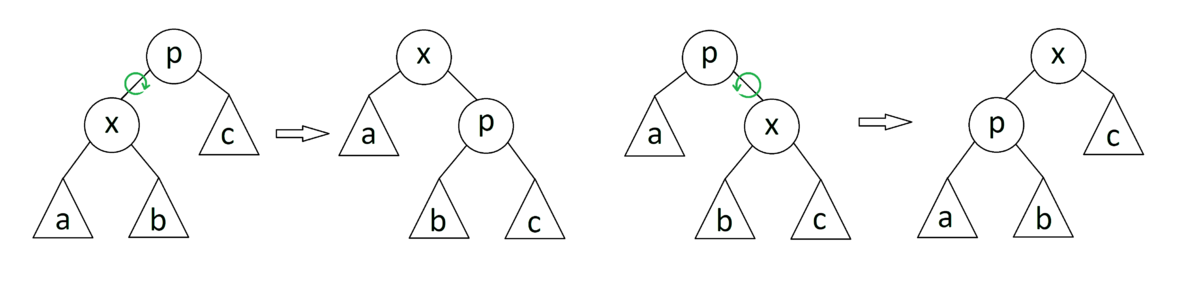
\includegraphics[width = 10cm]{pix/splay_zig.png}

    \textbf{Замечание } Это то же самое, что левый (правый) маленький поворот

    \item\textbf{zig-zig}

    Если p — не корень дерева, а x и p — оба левые или оба правые дети, то делаем поворот ребра (p,g), где g отец p, а затем поворот ребра (x,p).

    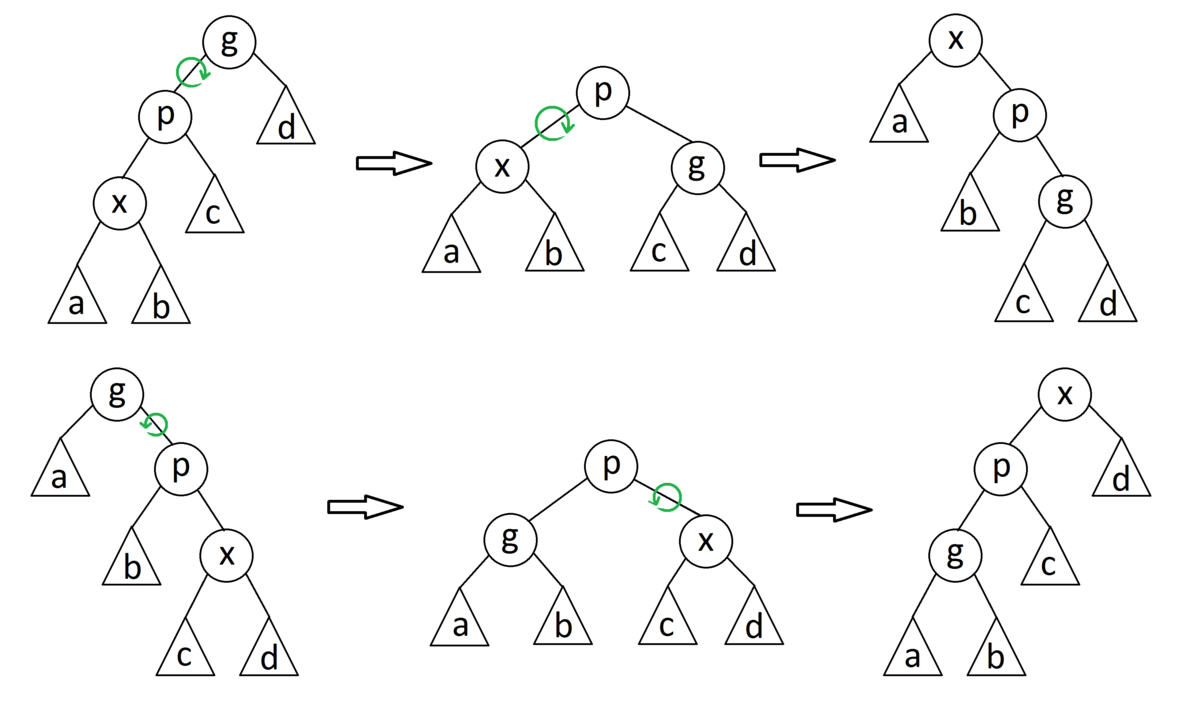
\includegraphics[width = 10cm]{pix/splay_zig_zig.png}

    \item \textbf{zig-zag}

    Если p — не корень дерева и x — левый ребенок, а p — правый, или наоборот, то делаем поворот вокруг ребра (x,p), а затем поворот нового ребра (x,g), где g — бывший родитель p.

    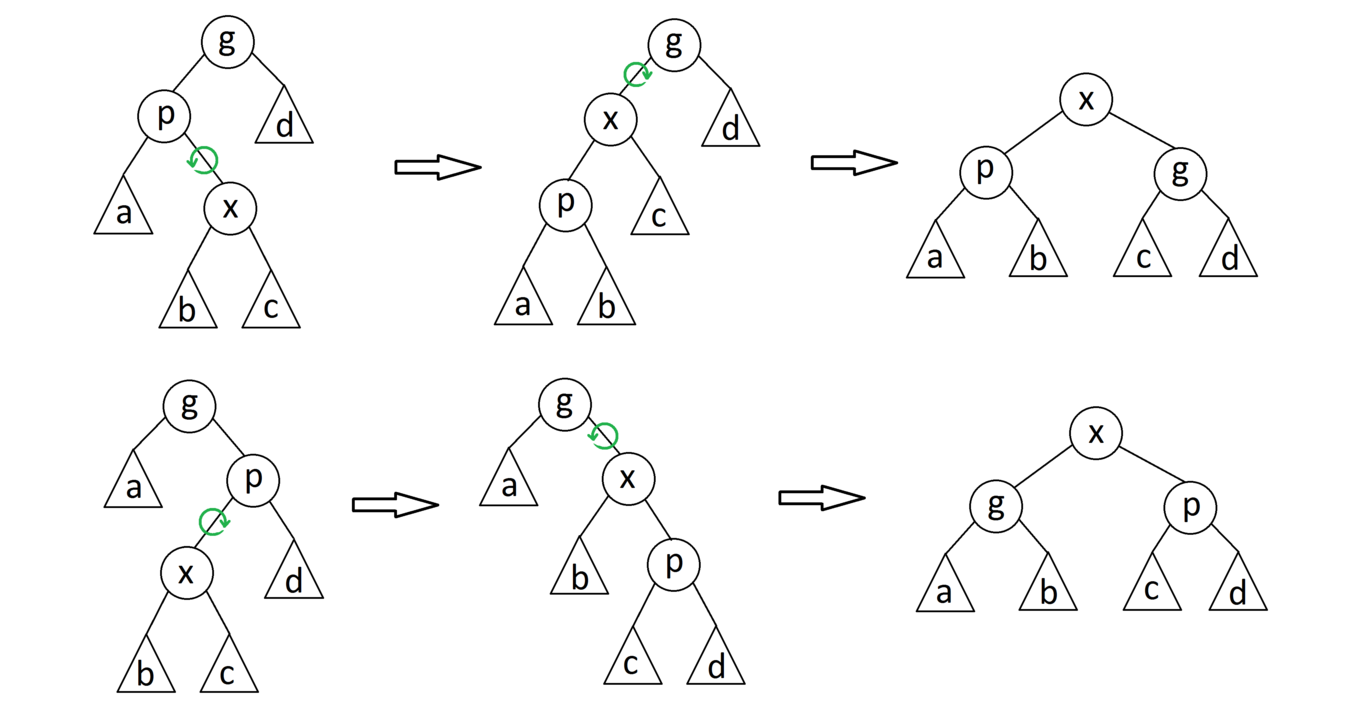
\includegraphics[width = 10cm]{pix/splay_zig_zag.png}

     \textbf{Замечание.} Это то же самое, что левый (правый) большой поворот
\end{itemize}

Таким образом, чтобы поднять элемент X  в корень дерева, нужно произвести какую-то комбинацию zig-zig и zig-zag, а в конце, возможно, сделать один zig.
\subsection{Амортизированное время работы операции splay с помощью метода потенциалов.}

Для некоторого состояния структуры S вводим потенциал $\Phi(S)$— это функция от состояния структуры.

Изначально потенциал равен $\Phi_0$, а после выполнения i-й операции - $\Phi_i$.
$t_i$ - реальное время работы i-й операции, тогда амортизированное время работы операции:  $a_i$ = $t_i$ + $\Phi_i - \Phi_{i-1} $.

Тогда $a_1 + a_2 + ... + a_q  = t_1 + t_2 + ... + t_q + (\Phi_1 - \Phi_0) + (\Phi_2 - \Phi_1) + ... + (\Phi_q - \Phi_{q-1}) = \displaystyle\sum_{i=1}^{q} t_i + \Phi_q - \Phi_0$

Если $\Phi_q - \Phi_0 \geq 0$, то получаем то, что нам нужно:

$\displaystyle\sum_{i=1}^{q} t_i \leq \displaystyle\sum_{i=1}^{q} a_i$ 

Т.е. реальное время работы не превосходит амортизированного.

\subsection*{Оценка времени работы операции splay}
\Th Амортизированное время работы операции  splay есть О(log(n)).

\Proof Положим S(x) - количество элементов в поддереве x (x  включается в поддерево),

r(x) = $\log_{2}{S(x)}$

$\Phi(x) = \displaystyle\sum_{x\,\in\,tree} r(x)$

Давайте рассмотрим i-ую операцию, на которой происходит splay(x)
Покажем, что $a_i \leq 1 + 3( r'(x) - r(x)) \leq 1 + 3\log_{2}{n}$, где $r'(x)$ - ранг x  в новом дереве, $r(x)$ - ранг x  в старом дереве.

После операции splay x переходит в корень, поэтому $r'(x) = \log_{2}{n}$ $\Longrightarrow$ $a_i \leq O(\log_{2}{n})$

Теперь рассмотрим амортизированное время работы операций zig, zig-zig, zig-zag:
\begin{itemize}
\item \textbf{zig}

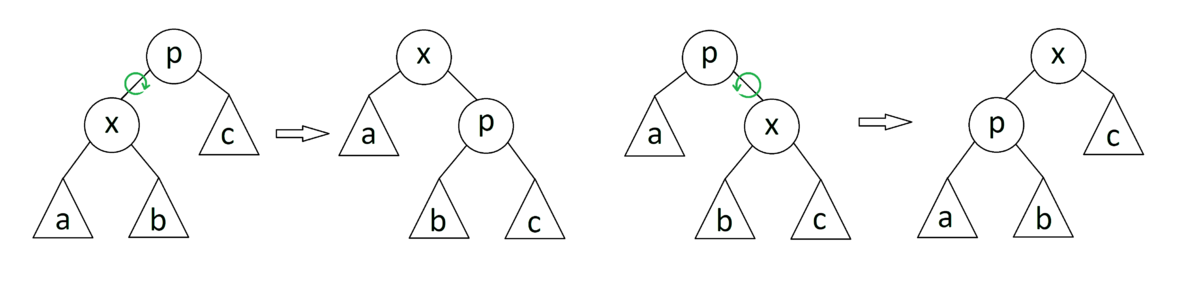
\includegraphics[width = 10cm]{pix/splay_zig.png}

$a(zig) = 1 + r'(x) + r'(p) - r(x) - r(p)$

$r'(p) \leq r(p)    \Longrightarrow     a(zig) \leq 1 + r'(x) - r(x) \leq 1 + 3(r'(x) - r(x))$

\item \textbf{zig-zig}

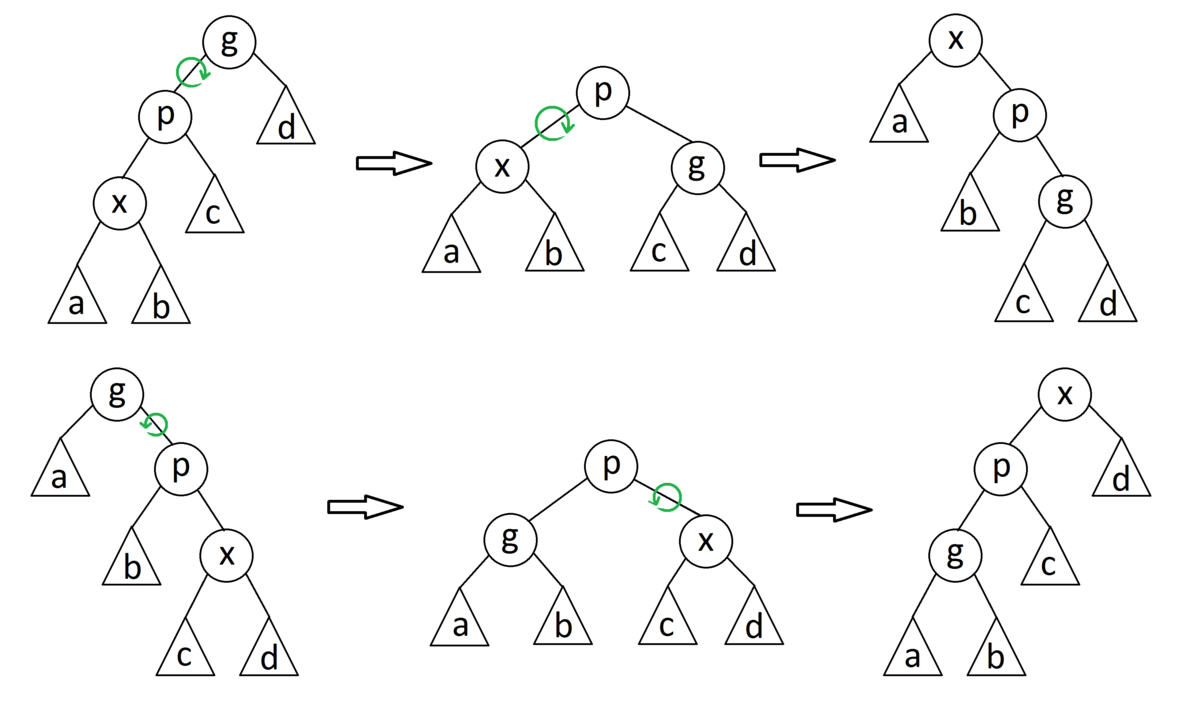
\includegraphics[width = 10cm]{pix/splay_zig_zig.png}

$a(zig-zig) = 2 + r'(x) + r'(p)  + r'(g)- r(x) - r(p) - r(g)$

$r'(x) = r(g), r(p) \geq r(x), r'(p) \leq r'(x)  \Longrightarrow $

$a(zig-zig) \leq 2 + r'(x)  + r'(g)- 2r(x) $

Проверим, выполняется ли, что 

$ 2 + r'(x)  + r'(g)- 2r(x) \leq 3(r'(x) - r(x))$

$ r'(g) + r(x) - 2r'(x) \leq -2$


$\displaystyle \log_{2}{\frac{S'(g)}{S'(x)}} + \log_{2}{\frac{S(x)}{S'(x)}} \leq -2$

$\displaystyle \frac{S'(g)}{S'(x)} = a, \frac{S(x)}{S'(x)} = b $

Покажем, что $a + b \leq 1$

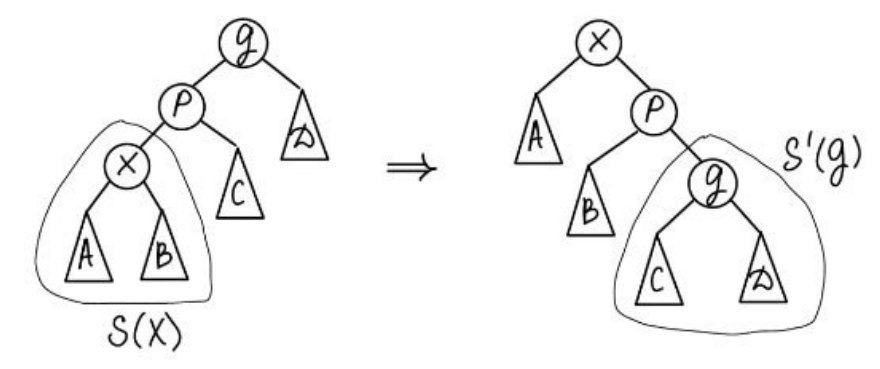
\includegraphics[width = 7cm]{pix/47-50_zzp.jpg}

Понятно, что каждый блок содержит меньше элементов, чем S'(x), при этом они не пересекаются, поэтому $a + b \leq 1$. Из неравенства о среднем геометрическом $ab \leq 1/4$ $ \Longrightarrow $ неравенство верно.

\item \textbf{zig-zag}

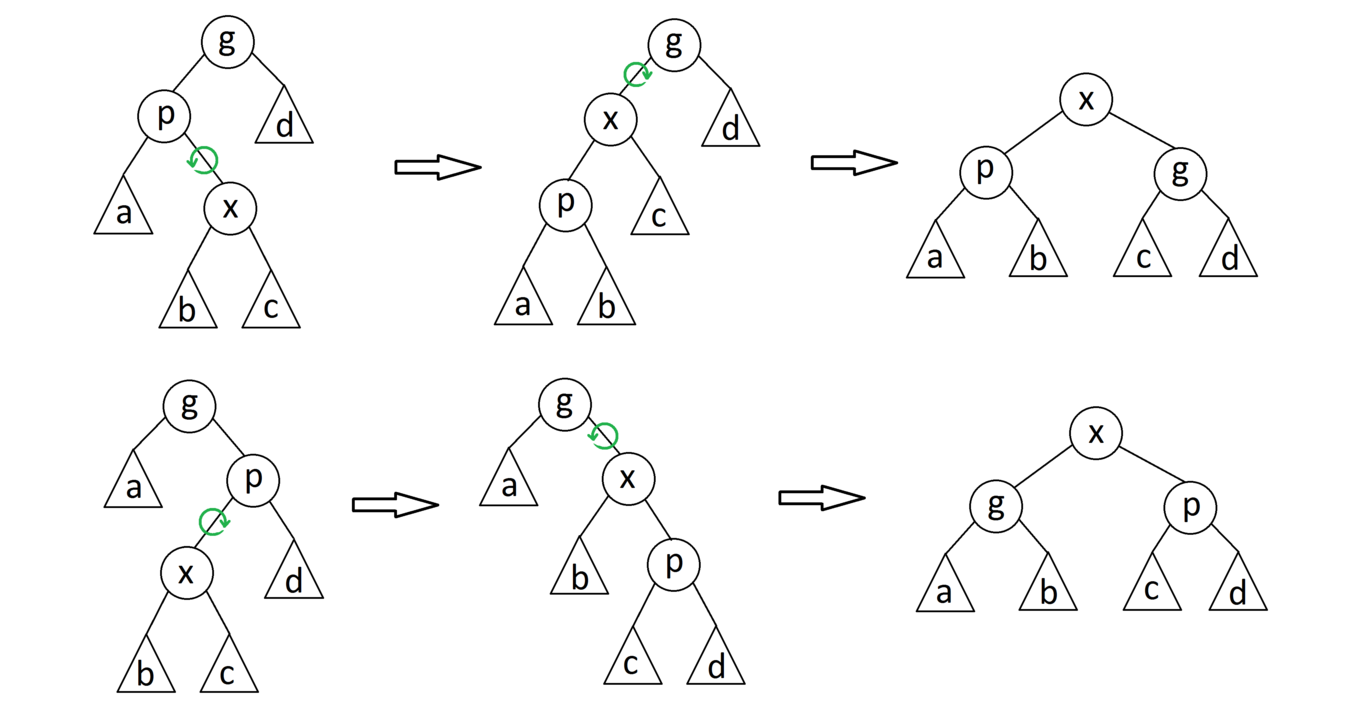
\includegraphics[width = 10cm]{pix/splay_zig_zag.png}

$a(zig-zag) = 2 + r'(x) + r'(p)  + r'(g)- r(x) - r(p) - r(g)$

$r'(x) = r(g), r(p) \geq r(x) \Longrightarrow $

$a(zig-zag) \leq 2 + r'(p) + r'(g) - 2r(x)$

Проверим, выполняется ли, что 

$ 2 + r'(p) + r'(g) - 2r(x) \leq 2(r'(x) - r(x))$    $\Leftrightarrow$

$r'(p) + r'(g) - 2r'(x) \leq -2$
$\Leftrightarrow$

$ \log_{2}{\frac{S'(g)}{S'(x)}} + \log_{2}{\frac{S'(p)}{S'(x)}} \leq -2$

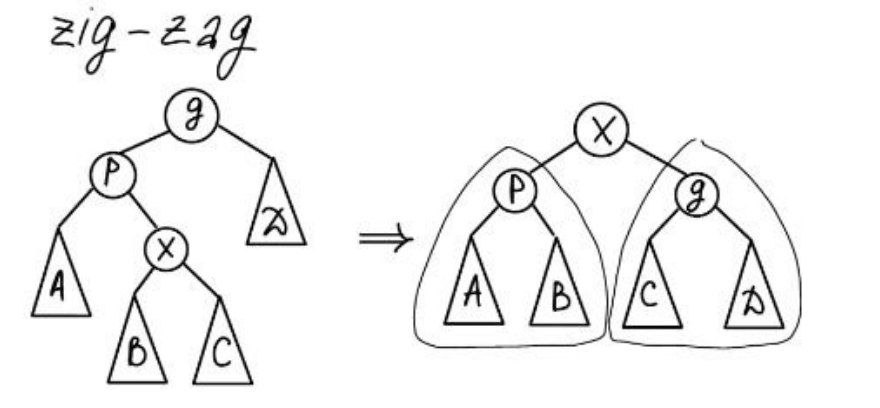
\includegraphics[width = 7cm]{pix/47-50_zzp@.jpg}

Тут доказывается аналогично предыдущему пункту. Таким образом

$ 2 + r'(p) + r'(g) - 2r(x) \leq 2(r'(x) - r(x)) \leq 3((r'(x) - r(x)))$

\end{itemize}

Отсюда следует, что каждая операция выполняется не более чем за $1 + 3( r'(x) - r(x))$. Сложим все операций, которые выполняли для того чтобы поднять элемент x:

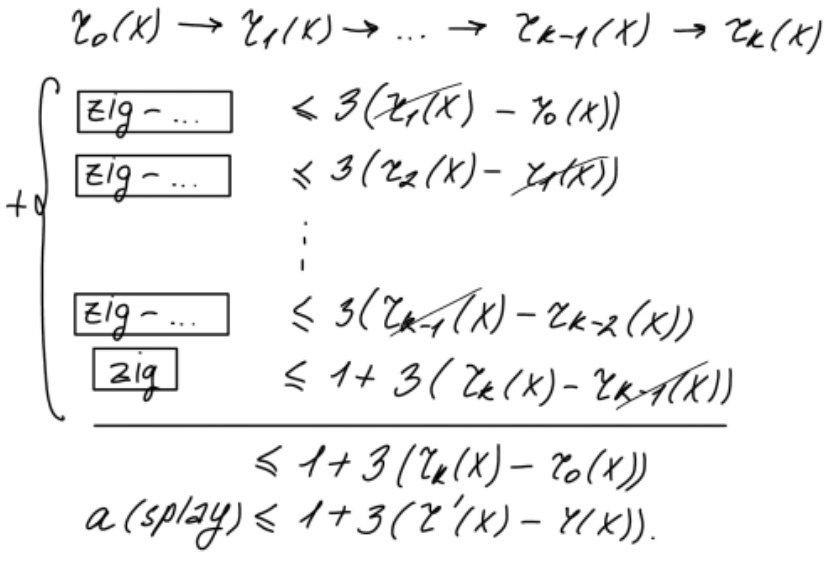
\includegraphics[width = 10cm]{pix/47-50_zzzend.jpg}

В результате получим то, что нужно.
\Endproof

\pagebreak

\section{29. Splay-дерево. Определение операции Splay. Выразимость остальных операцияй через Splay.}
\subsection{Splay-дерево: реализация insert, erase и find, связь с операцией splay, оценка времени работы.}

\subsection*{Insert }

Находим, куда нам нужно вставить x в дереве, запускаем splay от этого элемента, как это делали в обычном дереве, а потом вызываем splay от x. 

\textit{Асимптотика: Время insert ограниченно сверху временем работы splay. Амортизированное время работы: $O^*(\log(n))$}

\subsection*{Erase }

Поступаем точно так же, как делали в обычном бинарном дереве: разбиваем ситуацию на 3 случая, в зависимости от количества детей, но после того, как удаление произошло, запускаем splay от самой глубокой посещенной вершины.

\textit{Асимптотика: Время erase ограниченно сверху временем работы splay. Именно поэтому мы делаем splay от самой глубокой посещенной вершины. Амортизированное время работы: $O^*(\log(n))$}

\subsection*{Find }

Эта операция выполняется как для обычного бинарного дерева поиска, только после нее запускается операция splay от найденного элемента.

\textit{Асимптотика: как и в предыдущих случаях, время работы оценивается сверху временем работы splay, поэтому: амортизированное $O^*(log(n))$}

\pagebreak

\section{30. Задачи RMQ, RSQ. Постановки online/offline, static/dynamic.}
\Def Static - элементы во время запросов \textbf{не меняются}. То есть, нет такого запроса, который требует изменить что то в данных и продолжать работать с обновленными.

\Def Dynamic - элементы во время запросов \textbf{могут изменяться}.\\

\Def Online - все запросы \textbf{не известны} заранее и поступают только после ответа на предыдущий.

\Def Offline - все запросы \textbf{известны} заранее. Появляется возможность считать все запросы и ответить на них в удобном порядке.\\

\Def RMQ(Range Min Query) - запрос минимума на подотрезке

\Def RSQ(Range Sum Query) - запрос суммы на подотрезке

\Examples

static online(и offline тоже) RSQ - решается с помощью \hyperlink{prefsum}{префиксных сумм}

static online RMQ - решается с помощью \hyperlink{sparse table}{sparse table}

всевозможные варианты этих задач решает \hyperlink{segtree}{дерево отрезков}
\pagebreak

\hypertarget{sparse table}{}
\section{31. Разреженная таблица. Область применимости. Построение. Ответ на запрос.}
\Def Операция f идемпотентна, если $\forall a \rightarrow f(a,\,a)\,=\,a$.

\Def Разреженная таблица или Sparse Table — двумерная структура
данных ST[i][j], построенная на бинарной идемпотентной операции F, для которой выполнено следующее:

\begin{center}
$ST[i][j] = F(A[j],\,A[j + 1],\,\dots,\,A[j + 2^i - 1]),\,i \in [0 \dots log_2\,N]$
\end{center}

$ST[i][j] =
\begin{cases}
F(ST[i-1][j],\,ST[i-1][j+2^{i-1}])\text{, если i > 0}\\
A[j]\text{, если i = 0}
\end{cases}$

Заметим, что в этой таблице хранятся результаты функции F на всех отрезках, длины которых равны степеням двойки.
Выполним сначала предподсчет, суть которого в вычислении массива $floor\_log[i]\,=\,\lfloor log_2 i \rfloor$. Теперь заметим, что для отрека [l, r] верно, что

{\centering $F(A[l],\,A[l + 1],\,\dots,\,A[r]) = F(ST[i][l],\,ST[i][r - 2^i + 1])$,\par}
где $i\,=\,floor\_log [r - l + 1]$

\drawsomelarge{pix/sparse_table.png}

\textbf{Асимптотика}

В таблице хранятся результаты функции F на всех отрезках, длины
которых равны степеням двойки. Однако для каждого $j \in [0 \dots log_2\,N]$
таких отрезков не более N, откуда потребляемая память составит
$O(N\,log\,N)$.\\
Теперь время построения. Заметим, что каждая ячейка
пересчитывается за $O(1)$, откуда время построения $O(N\,log\,N)$.\\
И последнее — ответ на запрос. Заметим, что это всего лишь
вычисление функции от двух значений, что работает за $O(1)$.

\subsubsection*{Область применимости}

Можно решать static RMQ

% RSQ ни в каких постановках задачи нельзя решать, т.к. сумма не идемпотентна.

RSQ за $O(1)$ ни в каких постановках задачи нельзя решать, т.к. сумма не идемпотентна. Однако RSQ можно решить с помощью SparseTable, если разбить запрос суммы на отрезки, длины которых - это степени двоек. Таких отрезков будет $\log_2{n}$ - в силу представления числа в двоичной системе счисления, а ответ для каждого из таких отрезков уже предподсчитан в SparseTable (По определению), значит получаем асимптотику $O(\log n)$ на запрос RSQ.   

\pagebreak

\hypertarget{segtree}{}
\section{32. Дерево отрезков. Область применимости. Построение. Случай отсутствия обновлений на подотрезке. Изменение в точке. Ответ на запрос.}
\Def Дерево отрезков (англ. Segment tree) — это структура данных, которая позволяет за асимптотику $O(log(n))$ реализовать любые операции, определяемые на множестве, на котором данная операция ассоциативна, коммутативна и имеет нейтральный элемент относительно этой операции.

В частности, задачи RSQ/RMQ, как правило, решается с использованием этой структуры данных.

\begin{center}
 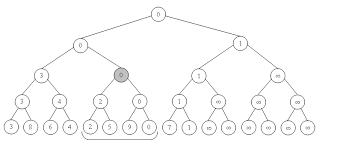
\includegraphics[width = 10cm]{pix/stree.png}    
\end{center}

\subsubsection{Построение}
Опишем нерекурсивное построение дерева на массиве длины N.

\begin{enumerate}
    \item Будем считать, что $log_2\,N \in \N$, иначе дозаполним до степени двойки нейтральными элементами.
    \item Заведем массив длины $2N - 1$, последние $N$ элементов будут элементами исходного массива.
    \item Первые $N - 1$ элементов заполним следующим образом:\\
    $t[i]\,=\,F(t[2i + 1],\,t[2i + 2])$ (заполнение от элемента с номером N - 2 и до 0 в цикле).
\end{enumerate}

\subsection*{Изменение в точке}

Пусть необходимо обновить элемент с индексом i.
\begin{enumerate}
    \item Найдем в дереве лист, отвечающий за i-й элемент. Это $(N - 1 + i)$-й.
    \item Индекс родителя $\lfloor \frac{N - 2 + i}{2} \rfloor$ (Если корень в вершине с номером 0)
    \item Обновляем значение в родителе через результаты на деревьях.
    \item Повтори, пока не обновил корень.
\end{enumerate}

\subsubsection*{Ответ на запрос}
Пусть мы находимся в узле, отвечающего за подотрезок $[l,\,r]$, а изначальный запрос был $[L,\,R]$.

\begin{enumerate}
    \item Если $[l,\,r] \cap [L,\,R] = \varnothing$, то вернем нейтральный элемент.
    \item Если $[l,\,r] \subseteq [L,\,R]$, то вернем значение в узле.
    \item Иначе вернем результат операции с детей.
\end{enumerate}

\textbf{Асимптотика} Заметим, что на каждом уровне раскрываться вниз могут не более двух узлов, так как только крайние могут порождать дочерние запросы. Следовательно, время работы $O(log\,N)$.

\pagebreak

\section{33. Дерево отрезков. Область применимости. Построение. Случай наличия обновлений на подотрезке. Изменение в точке. Ответ на запрос.}
\subsection*{Случай наличия обновлений на подотрезке}

\textbf{Идея отложенных операций} 
Применим следующий трюк: если нам нужно обновить значение подотрезка, то мы отложим эту операцию до востребования. Запомним в соответствующих вершине/блоке, что мы должны в будущем сделать обновление в потомков. Если нам вдруг понадобится значение, лежащее в вершине/блоке, то мы посчитаем его так, как будто мы обновили отрезок, а напоминание о том, что надо сделать со всеми элементами, мы "протолкнем"в потомков.

\Def Операцией группового обновления ch будем называть запрос, в
ходе которого применяется на подотрезке операция $ch(\cdot,\,val)$.

Свойства на операцию ch, если op — операция запроса на отрезке.

\begin{enumerate}
    \item Существование нейтрального элемента
    \item Ассоциативность: $ch(a,\,ch(b,\,c))\,=\,ch(ch(a,\,b),\,c)$
    \item Дистрибутивность: $ch(op(a,\,b),\,c)\,=\,op(ch(a,\,c),\,ch(b,\,c))$
\end{enumerate}

\Def Несогласованность -- величина, с которой надо выполнить операцию op, чтобы получить корректный результат.

В каждый момент времени в узле необязательно лежит истинное значение op на отрезке. Но к моменту запроса будем осуществлять проталкивание несогласованности.

\begin{lstlisting}
void push(int node) {
  tree[2 * node + 1].lazy = ch(tree[2 * node + 1].lazy, tree[node].lazy);
  tree[2 * node + 2].lazy = ch(tree[2 * node + 2].lazy, tree[node].lazy);

  tree[node].d = ch_neutral
}
\end{lstlisting}

Вызывать push надо каждый раз, когда мы обращаемся к вершине, которая могла
быть изменена

\subsubsection{Запрос на группового обновления}

\begin{lstlisting}
void update(int node, int a, int b, T val) {
  l = tree[node].left
  r = tree[node].right

  if ([l, r) is subset [a, b)) {
    tree[node].lazy = ch(tree[node].lazy, val);
    return;
  }
  push(node);

  update(2 * node + 1, a, b, val);
  update(2 * node + 2, a, b, val);
  tree[node].val = op(
    ch(tree[2 * node + 1].val, tree[2 * node + 1].lazy),
    ch(tree[2 * node + 2].val, tree[2 * node + 2].lazy),
  );
}
\end{lstlisting}

\Alg
\begin{enumerate}
    \item Первая часть посвящена разбиению на объединение подотрезков. Если подмножество, то накапливаем несогласованность.
    \item Проталкивание.
    \item Обновляем детей.
    \item Обновляем результат. Заметим, что у нас несогласованность уже нейтральная, так что надо просто собрать op с «истинных» значений у детей.
\end{enumerate}

\subsection{Ответ на запрос}

Выполняется аналогично групповому обновлению

\begin{lstlisting}
int query(int node, int a, int b) {
  l = tree[node].left
  r = tree[node].right

  if ([l, r) is subset [a, b)) {
    return ch(tree[node].val, tree[node].lazy);
  }
  push(node);

  answer = op(
    query(2 * node + 1, a, b),
    query(2 * node + 2, a, b),
  );

  tree[node].val = op(
    ch(tree[2 * node + 1].val, tree[2 * node + 1].lazy),
    ch(tree[2 * node + 2].val, tree[2 * node + 2].lazy),
  );
  return answer;
}
\end{lstlisting}

\pagebreak

\section{34. Декартово дерево по неявному ключу. Задача о развороте подотрезка.}
\Task Пусть у нас есть массив $A[1 : n]$.
Требуется уметь выполнять следующие операции: \\

\begin{enumerate}
    \item Insert(x, pos) - вставить элемент x после элемента с позицией pos.
    \item Erase(pos) - удалить элемент с позицией pos.
    \item Посчитать сумму элементов с l по r.
\end{enumerate}

\textbf{Структура ДДНК.}
При реализации декартова дерева по неявному ключу модифицируем \textit{декартово дерево}. А именно, оставим в нем только приоритет Y, а вместо ключа X будем использовать следующую величину: \textbf{количество элементов в нашей структуре, находящихся левее нашего элемента}. Иначе говоря, будем считать ключом порядковый номер нашего элемента в дереве, уменьшенный на единицу. 

\textbf{Вспомогательная величина.}
Основная идея заключается в том, что такой ключ X сам по себе нигде не хранится. Вместо него будем хранить вспомогательную величину T.size(): количество вершин в поддереве нашей вершины (в поддерево включается и сама вершина). 

\subsection{Операции:}
\begin{enumerate}
    \item \textbf{Merge} будет как в обычном декартовом дереве (так как он смотрит исключительно на приоритеты), но с поддержкой значения $T.size()$.
    \item \textbf{Split(T, k)} (отрезать от дерева первые $k$ вершин). Также известно, что в левом поддереве вершины находится $l$ вершин, а в правом $r$. Рассмотрим все возможные случаи:
    \begin{enumerate}
        \item $l \geq k$. В этом случае нужно рекурсивно запустить процедуру \texttt{split} от левого сына с тем же параметром $k$. При этом новым левым сыном корня станет правая часть ответа рекурсивной процедуры, а правой частью ответа станет корень.
        \item $l < k$. Случай симметричен предыдущему. Рекурсивно запустим процедуру \texttt{split} от правого сына с параметром $k - l - 1$. При этом новым правым сыном корня станет левая часть ответа рекурсивной процедуры, а левой частью ответа станет корень.
\begin{lstlisting}
(Treap, Treap) Split(Treap treap, int k)
  if (treap == null) {
    return (null, null)
  }
  int left = treap.left.size
  if (left >= k) {
    (t1, t2) = Split(treap.left, k)
    treap.left = t2
    Update(treap)
    return (t1, treap)
  }
  (t1, t2) = Split(treap.right, k - l - 1)
  treap.right = t1
  Update(treap)
  return (treap, t2)
}
\end{lstlisting}
    \end{enumerate}
\item \textbf{Insert(T, k, value)} аналогично декартову дереву, вместо ключа - индекс после которого необходимо вставить элемент.
\end{enumerate}

\subsection{Задача о развороте подотрезка}

Стоит заметить, то о чём будем далее рассказываться очень похоже на массовые операции в Дереве Отрезков (В особенности, проталкивание).

\vspace{1cm}

Чтобы решить эту задачу, будем хранить булевую переменную в каждой вершине. Назовём её toReverse. 
\begin{equation*}
    toReverse = 
    \begin{cases}
        True, \text{ если нужно развернуть подотрезок, состоящий из элементов поддерева вершины}\\
        False, \text{ иначе}
    \end{cases}
\end{equation*}
\textbf{Проталкивание:} допустим, мы находимся в вершине $v$ (Неважно, в merge или split). В таком случае, нам нужно протолкнуть toReverse в детишек. Если toReverse $= False$, то ничего не делаем, иначе делаем $v.LeftSon.toReverse = v.LeftSon.toReverse\, \oplus \,v.toReverse$ (То есть мы ксорим булевую переменную левого сына с нашей булевой переменной). То же самое делаем и для правого сына, после чего обнуляем наш toReverse, так как проталкивание выполнено. Также нужно непосредственно swap-нуть сыновей (То есть, буквально написать $std::swap(v.LeftSon, v.RightSon)$)

\textbf{(*)} Может возникнуть вопрос: почему мы именно ксорим? Дело в том, что если в сыне и так было $toReverse = True$, то ещё один разворот "нейтрализует"\ его и по итогу ничего разворачивать не нужно, то есть нужно сделать $toReverse = False$. А если $toReverse$ сына $= False$, то как раз нужно просто сделать $toReverse = True$, чтобы не писать $if$-ы, мы воспользовались ксором.

\textbf{Обработка запроса о развороте подотрезка $[l, r]$:}
\begin{enumerate}
    \item Вырезаем отрезок $[l, r]$ с помощью split().
    \item В корне получившейся "вырезки" делаем $v.toReverse = v.toReverse \bigoplus 1$. Это мы делаем из тех же рассуждений, что и \textbf{(*)}
    \item Склеиваем всё обратно
\end{enumerate}
\pagebreak


\section{35. Хеш-функция. Коллизия. Хеш-таблица и основные операции. Хеш-таблица на цепочках (время
работы б/д).}
\subsection*{Хеш-функция.}

\Def Пусть $U$ - множество рассматриваемых объектов, тогда $h: U \rightarrow \{0, 1, \dots, m - 1\}$ называется хеш-функцией.

\subsection*{Коллизия.}

\Def Элементы $x, y \in U$, где $x \neq y$ образуют \textit{коллизию}, если $h(x) = h(y)$.

\subsection*{Хеш-таблица.}

Заведем массив размера $|h(U)|$ и будем класть булев флаг в ячейку $h(x)$, если элемент x 
есть в массиве. 

Минусы:
\begin{itemize}
    \item Огромные затраты памяти $\rightarrow$ можно завести массив размера $m$ и класть элемент по индексу $h(x) \% m$.
    \item Коллизии.
\end{itemize}

\subsection*{Операции}
\begin{itemize}
    \item Insert - добавляет элемент.
    \item Delete - удаляет элемент.
    \item Contains (Random access) - проверка на наличие элемента в таблице.
\end{itemize}

\subsection*{Хеш-таблица на цепочках.}

\Def Бакет (bucket) - нечто, хранящее все элементы, образующие коллизию.

Вместо обычной хеш-таблицы заведем хеш-таблицу на цепочках. Вместо булевых флагов в ячейках $h(x)$ будем хранить цепочки (бакеты) с элементами которые образовали коллизию. То есть получим массив цепочек, где все операции работают за длину цепочки.

\subsection*{Время работы.}

Если соблюдать ограничение на \textit{load factor}, то сложность всех операций составит $\mathcal{O}(1)$ в среднем. 
\newline 
$\rightarrow$ Вставка, удаление и поиск в среднем за $\mathcal{O}(1)$.

\Note \textit{load factor} - коэффициент загруженности (подробнее в след. билете).

\pagebreak

\section{36. Гипотеза простого равномерного хеширования. Математическое ожидание длины цепочки.}
\subsection*{Гипотеза простого равномерного хеширования.}

Проблема хеш-таблицы на цепочках - неравномерная длинна цепочки из-за неравномерности возникновения коллизии. $\Rightarrow$ Хочется минимизировать максимальную длину цепочки, то есть добиться того чтобы функция равномерно распределяла ключи по бакетам.

Пусть $\mathcal{H} = \{h:U \rightarrow \{0, 1, \dots, k - 1\} \}$ - множество хеш-функций.

\Note $U \subset \mathbb{N}$ и $|U| < \infty$, то есть $U = \{0, 1, \dots, n - 1\}$.

Определим случайную функцию как то, что образ каждого ключа - это случайный элемент из множества $\{0, 1, \dots, k - 1\}$.

\Note Неприменимо на практике, т.к. требует $\mathcal{O}(|U|\log|h(U)|)$ памяти на хранение такого отображения.

\Def Модель, описанная выше, называется \textit{простое равномерное хеширование} (\textit{simple uniform hashing}).

\subsection*{Математическое ожидание длины цепочки.}

Величина $L_q$ - длинна цепочки по ключу $q$.\newline
Пусть построена таблица для ключей $k_1, \dots, k_n$, тогда 

\begin{center}
{\large $L_q = \sum\limits_{i = 1}^{n} I(h(q) = h(k_i))$}
\end{center}

Посчитаем матожидание длины цепочки.

\begin{center}
{\large $\mathbb{E} L_q = \mathbb{E}\sum\limits_{i = 1}^{n} I(h(q) = h(k_i)) = \sum\limits_{i = 1}^{n} P(h(q) = h(k_i))$}
\end{center}

Посчитаем вероятность.

\begin{center}
    {\large $ P(h(x) = h(y)) =
        \begin{cases}
        1, \ x = y\\
        \frac{1}{k}, \ x \neq y 
    \end{cases} $}
\end{center}

С учетом того что все ключи различны, получаем, что

\begin{center}
{\large $\mathbb{E} L_q = \mathbb{E} \sum\limits_{i = 1}^{n} I(h(q) = h(k_i)) = \sum\limits_{i = 1}^{n} P(h(q) = h(k_i)) \leq 1 + \frac{n}{k}$}
\end{center}

\Def Коэффициентом загруженности \textit{(load factor)} называют величину $\alpha = \frac{n}{k}$.

\Note Из оценок выше можно задать константу $C$ такую, что всегда $\alpha < C$. Тогда в среднем сложность операций составит $\mathcal{O}(1)$.

\pagebreak

\section{37. Задача о наибольшей возрастающей подпоследовательности. Решение за квадратичное время.}
\Task Дан массив $a_{1}, \dots , a_{n}, a_{i} \in \R$. Необходимо извлечь наибольшую по
длине возрастающую подпоследовательность. То есть найти такие
индексы $1 \Le i_{1} < i_{2} < . . . < i_{k} \Le n$, что $a_{i_{j}} < a_{i_{j+1}}$ и $k$ максимально за $\mathcal{O}(n^2)$.

\Solution Решение задачи базируется на идее динамического программирования.

1) \textit{Смысл dp.} dp[i] - длина НВП, заканчивающейся на $a_{i}$.

2) \textit{База dp.} dp[:] = 1.

3) \textit{Ф-ла пересчета.} dp[i] = $1 + \max \limits_{j<i,a_j<a_i} dp[j]$.

4) \textit{Порядок вычислений} \textit{for i = 2 \dots n}

5) \textit{Где ответ}  $\max \limits_{i} dp[i]$.

\Note Для того, чтобы получить саму подпоследовательность, необходимо восстановить порядок прохода. Это можно сделать, если на 3 шаге дополнительно хранить \texttt{ancestors[i] = j}.\\

Рассмотрим код:

\begin{lstlisting}
int LIS(int[] array, int len) {
  int[] dp(len + 1, 1);
  for (int i = 2 ... n) {
    for (int j = 1 ... i) {
      if (array[i] > array[j]) {
        dp[i] = max(dp[i], 1 + dp[j]);
      }
    }
  }
  return max(dp);
}
\end{lstlisting}
\pagebreak

\section{38. Задача о наибольшей возрастающей подпоследовательности. Решение за $O(N log N)$, где $N$ —
длина последовательности.}
\Task Дан массив $a_{1}, \dots , a_{n}, a_{i} \in \R$. Необходимо извлечь наибольшую по
длине возрастающую подпоследовательность. То есть найти такие
индексы $1 \Le i_{1} < i_{2} < . . . < i_{k} \Le n$, что $a_{i_{j}} < a_{i_{j+1}}$ и $k$ максимально за $\mathcal{O}(n\,log(n))$.

\textbf{Решение 1:}

1) Сформируем пары $\begin{pmatrix}
a_{i}\\
i
\end{pmatrix}$

2) Отсортируем их по возрастанию $a_{i}$, при равенстве - по убыванию $i$. Тогда, ограничение $a_{j} < a_{i}$ естественно выполняется.

3) \textit{Смысл dp.} dp[i] - длина НВП, заканчивающейся на $a_{i}$.

4) \textit{База dp.} dp[:] = 0.

5) \textit{Пересчёт, изменение по индексу} dp[i] = $1 + \max \limits_{j < i}(dp[j])$ - Можно посчитать с помощью \hyperlink{segtree}{дерева отрезков} за $\mathcal{O}(log(n))$.

6) \textit{Порядок вычислений. for ($a_i, i$) in sorted(pairs)} 

7) \textit{Ответ} лежит в dp[:].

\drawsomesmall{pix/picsol_nvp.jpg}

\textbf{Решение 2:}

1) \textit{Смысл dp.} dp[i] - минимальный элемент, на котором заканчивается последовательность длины $i$.

2) \textit{База dp.} dp[0] = $-\inf$, dp[1:] = $+\inf$.

3) \textit{Пересчёт} Место для $a_i$ можно найти бинпоиском. И правда, возрастающая подпоследовательность с ним может заканчиваться на это число только если оно больше последнего элемента, на которое заканчивается подпоследовательность без него, то есть оно может встать максимум на dp[k+1], где k - наибольший индекс элемента в dp, которое меньше чем $a_i$.

\begin{lstlisting}
int dp[n+1];
dp[0] = -inf;
for (int i = 1; i < n + 1; i++) {
  dp[i] = +inf;
}

for (int i; i < n; i++) {
  int left = 0;
  int right = n+1;
  while (left + 1 < right) {
    int mid = (left + right) / 2;
    if (dp[mid] < a[i]) {
      left = mid;
    } else {
      right = mid;
    }
  }

  dp[right] = a[i]
}
\end{lstlisting}
4) \textit{Порядок вычислений. for i in 0 ... n} 

5) \textit{Ответ} индекс последнего элемента, который лежит в dp, меньший $+inf$.
\pagebreak

\section{39. Задача о наибольшей общей подпоследовательности.}
\Task Даны два массива $a_{1}, \dots, a_{n}$ и $b_{1}, \dots, b_{m}$. Необходимо извлечь
наибольшую по длине общую подпоследовательность. То есть найти такие индексы $1 \Le i_{1} < \dots < i_{k} \Le n$ и $1 \Le j_{1} < \dots < j_{k} \Le m$, что $a_{i_{q}} = b_{j_{q}}$ и $k$ максимально.

\Solution Решение задачи базируется на идее динамического программирования.

1) \textit{Смысл dp.} dp[i][j] - длина НОП для $a[: i]$ и $b[: j]$.

2) \textit{База dp.} dp[:][:] = 0.

3) \textit{Ф-ла пересчета.} $dp[i][j] = 
\begin{cases}
1 + dp[i-1][j-1], & \text{если } a_i = b_j, \\
\max(dp[i-1][j], dp[i][j-1]), & \text{иначе}
\end{cases}
$

4) \textit{Порядок вычислений} \textit{for i = 1 \dots n} \textit{for j = 1 \dots m}

5) \textit{Ответ} dp[n][m]


\pagebreak

\section{40. Задача о 0-1 рюкзаке.}
\Def Задача о рюкзаке — NP-полная задача комбинаторной оптимизации.

\subsection*{Постановка задачи (линейно-алгебраическая)}

Даны два вектора $w = (w_0, \dots , w_{n-1})$ и $c = (c_0, \dots , c_{n-1})$, оба вектора
из $\N^n$. Нужно построить битовый вектор $b \in \{0,\,1\}^n$ такой, что

\begin{center}
    \large
    $\begin{cases}
    (w, b) \leq W\\
    (c, b) \rightarrow max
    \end{cases}$
\end{center}

\subsection*{Постановка задачи (классическая)}

Есть $n$ предметов, каждый из них имеет вес $w_i$ и стоимость $c_i$. Надо взять какие-то предметы в рюкзак так, чтобы их суммарный вес не превосходил $W$, а стоимость максимальна.

\subsection*{Решение за $O(nW)$}

\begin{enumerate}
    \item \textit{Смысл dp:} $dp[i][w]$ = максимальная ценность предметов, полученных из первых $i$ имеющихся предметов, с суммарным весом не превышающим $w$.
    \item \textit{База dp:} $dp[:][:]\,=\,0$
    \item \textit{Ф-ла пересчета:} $dp[i][w]\,=\,max
    \begin{cases}
        dp[i-1][w] & \text{, $i$-й предмет не берем}\\
        dp[i-1][w-w_i]\,+\,c_i  & \text{, $i$-й предмет берем}
    \end{cases}$
    \item \textit{Порядок вычислений} $for\,(i = 1 \dots n)\,\{\,for\,(w = 0 \dots W)\,\}$
    \item \textit{Ответ:} $dp[n][W]$
\end{enumerate}

\begin{lstlisting}
dp = [[0 for _ in range(W + 1)] for _ in range(n + 1)]

for i in range(1, n + 1):
  for j in range(W + 1):
    if w[i - 1] > j:  
      dp[i][j] = dp[i - 1][j]
    else:
      dp[i][j] = max(dp[i - 1][j], dp[i - 1][j - w[i - 1]] + v[i - 1])
\end{lstlisting}

\pagebreak

\section{41. Динамическое программирование на подотрезках. Задача об оптимальном перемножении матриц.}
\subsection*{Принцип ДП по подотрезкам}

Если имеется способ расчета ответ на задачу на основе ответов на подотреках, то выгодно применить ДП по подотрезкам.

То есть для решения таковой задачи надо сделать следующее.

\begin{enumerate}
    \item $dp[l,\,r]$ — ответ на задачу на подотрезке $[l,\,r]$
    \item Задать базу для отрезков длины 1, 2
    \item Определить функцию «слияния» ответов. То есть как получить из результата на подотрезках результат для всего отрезка.
\end{enumerate}

\subsection*{Квадратичное ДП по подотрезкам}

Данная постановка предполагает, что ответ для отрезка $[l,\,r]$ можно извлечь из отрезков $[l + 1,\,r]$, $[l,\,r - 1]$, $[l + 1,\,r - 1]$.

\subsubsection*{Пример задачи}

Есть строка $S$. Надо найти длину максимальной подпоследовательности палиндрома за $O(|S|^2)$.

\Solve

\begin{enumerate}
    \item \textit{Смысл dp:} $dp[l][r]$ -- ответ для строки $S[l:r]$.
    \item \textit{База:} $dp[l][l] = 1$ и $dp[l][r] = 0$, если $r < l$.
    \item \textit{Ф-ла пересчета:} У нас могут быть две ситуации:
    \begin{itemize}
        \item Если $S[l] = S[r]$, то тогда нам выгодно оба эти символа докинуть в ответ и $dp[l][r]\,=\,dp[l + 1][r - 1]\,+\,2$.
        \item Если $S[l] \neq S[r]$, то тогда нам нет смысла учитывать данную букву, так что $dp[l][r]\,=\,max \{ dp[l + 1][r],\,dp[l][r - 1] \}$
    \end{itemize}
    \item \textit{Порядок вычислений:} $for\,(len=2 \dots n)\, \{ for\,(l = 0 \dots n) \}$
    \item \textit{Ответ:} $dp[0][|S| - 1]$
\end{enumerate}

\begin{lstlisting}
for (int len = 2; len < S.size(); ++len) {
  for (int l = 0; l < S.size() - len; ++l) {
    int r = l + len;
    if (S[l] == S[r]) {
      dp[l][r] = dp[l + 1][r - 1] + 2;
    } else {
      dp[l][r] = max(dp[l][r - 1], dp[l + 1][r]);
    }
  }
}
\end{lstlisting}

\subsection*{Кубическое ДП по подотрезкам}
Данная постановка предполагает, что ответ для отрезка $[l,\,r]$ можно извлечь из отрезков $[l,\,m]$, $[m + 1,\,r]$, где $m \in [l,\,r]$.

\subsubsection*{Пример задачи}
Есть строка S из разных типов скобок. Надо найти длину максимальной правильной скобочной подпоследовательности (ПСП) за $O(|S|^3)$.

\Solve

\begin{enumerate}
    \item \textit{Смысл dp:} $dp[l][r]$ -- минимальное число символов, которые надо удалить из $S[l:r + 1]$, чтобы получилась ПСП.
    \item \textit{База:} $dp[l][l] = 1$ и $dp[l][r] = 0$, если $r < l$.
    \item \textit{Ф-ла пересчета:} Посмотрим, что может произойти с $S[l]$
    \begin{itemize}
        \item Скобка будет удалена, тогда $dp[l][r]\,=\,dp[l+1][r]\,+\,1$.
        \item Скобка не будет удалена, тогда найдется парная ей скобка на
позиции $m \in [l + 1,\,r - 1]$.\\
Тогда итоговая ПСП на $S[l:r + 1]$ будет устроена как $(ans[l + 1 : m])ans[m + 1 : r + 1]$, то есть $dp[l][r]\,=\,dp[l + 1][m - 1]\,+\,dp[m + 1][r]$.\\
Тогда $dp[l][r]\,=\, \min\limits_{m \in (l,\,r)} ( dp[l + 1][m - 1]\,+\,dp[m + 1][r]$ ).
    \end{itemize}
    \item \textit{Порядок вычислений:} $for\,(len=2 \dots n)\, \{ for\,(l = 0 \dots n) \}$
    \item \textit{Ответ:} $|S|\,-\,dp[0][|S| - 1]$.
\end{enumerate}

\begin{lstlisting}
for (int len = 2; len < S.size(); ++len) {
  for (int l = 0; l < S.size() - len; ++l) {
    int r = l + len;
    dp[l][r] = dp[l + 1][r] + 1;
    for (int m = l + 1; m < r; ++m) {
      if (S[l] == '(' && S[m] == ')') {
        dp[l][r] = min(dp[l][r], dp[l + 1][m - 1] + dp[m + 1][r]);
      }
    }
  }
}
\end{lstlisting}

\subsection*{Задача об оптимальном перемножении матриц}

\Task Дана последовательность из $n$ матриц, требуется найти самый эффективный способ их перемножения.

У нас есть множество способов перемножить матрицы, потому что операция перемножения ассоциативна. Другими словами, нет разницы в каком порядке расставляются скобки между множителями, результат будет один и тот же. Однако, порядок в котором расставляются скобки между матрицами повлияет на количество арифметических операций, которые потребуются на вычисление ответа

Например, предположим, что $\dim{A}= 10 \times 30$, $\dim{B} = 30 \times 5$, $\dim{C} = 5 \times 60$. Тогда:\\
\tabДля $(A \times B)\times C$ будет $(10\times30\times5) + (10\times5\times60)  = 1500 + 3000 = 4500$ операций \\
\tabДля $ A \times(B \times C)$ будет $(30\times5\times60) + (10\times30\times60) = 9000 + 18000 = 27000$ операций.

Как мы видим, первый способ гораздо эффективней. 

\Solve 

Пусть $p_i$ -- размерность матрицы $i$

\begin{enumerate}
    \item \textit{Смысл dp:} $dp[l][r]$ -- минимальная стоимость вычисления матрицы $M_{l \dots r}$
    \item \textit{База:} $dp[l][r] = 
    \begin{cases}
    0, & l = r\\
    p_{l-1} \cdot p_{l} \cdot p_{l+1}, & r = l + 1\\
    \end{cases}$.
    \item \textit{Ф-ла пересчета:} $dp[l][r] = 
        \begin{cases}
        0, & l = r\\
        \min\limits_{m \in (l,\,r)} ( dp[l][m] + dp[m + 1][r] + p_{l-1} \cdot p_m \cdot p_r), & r < l
        \end{cases}$
    \item \textit{Порядок вычислений:} $for\,(len=2 \dots n)\, \{ for\,(l = 0 \dots n) \}$
    \item \textit{Ответ:} $dp[0][n-1]$
\end{enumerate}

\begin{lstlisting}
for (int i = 1; i < n; ++i) {
  dp[i][i] = 0;
}
for (int len = 2; len < n; ++len) {
  for (int l = 0; i < n - len; ++l) {
    int r = i + len;
    dp[l][r] = +inf;
    for (int m = l + 1; m < r; ++m) {
      dp[l][r] = min(dp[l][r], dp[l][m] + dp[m + 1][r] + p[l - 1] * p[m] * p[r]);
    }
  }
}
\end{lstlisting}

\pagebreak

\section{42. Матричное динамическое программирование. Подсчет k-го члена однородной линейной рекурренты n-го порядка за $O(n^3\,log\,k)$.}
\Def Линейным рекуррентным соотношением с постоянными коэффициентами (ЛРСПК) порядка n назовем соотношение вида $a_k = \sum\limits_{i=1}^n c_{i} a_{k-i}\,+\,f(k,a_{k-1},\dots,a_{k-n})$ с заданными $a_1, \dots , a_n$.

ЛРСПК называется однородным, если $f\, \equiv \,0$

\subsection*{Нахождение k-го члена однородной ЛРСПК n-го порядка за $O(n^3\,log\,k)$}

Запишем наши первые n членов последовательности в столбик $A_0 = \begin{pmatrix}
a_{n - 1}\\
a_{n - 2}\\
\vdots \\
a_0
\end{pmatrix}$

Так же выпишем следующую матрицу перехода:
$T = \begin{pmatrix}
c_1 & c_2 & c_3 & \cdots & c_{n - 1} & c_n\\
1 & 0 & 0 & \cdots & 0 & 0\\
0 & 1 & 0 & \cdots & 0 & 0\\
\vdots & \vdots & \vdots & ~ & \vdots & \vdots \\
0 & 0 & 0 & \cdots & 1 & 0\\
\end{pmatrix}$

Заметим, что умножив $T$ на $A_0$, мы получим столбик $A_1$ следующего вида: 
$A_1 = T \cdot A_0 = \begin{pmatrix}
a_{n}\\
a_{n - 1}\\
\vdots \\
a_1
\end{pmatrix}$
Аналогично, домножив $T$ на $A_1$, получим 
$A_2 = T \cdot A_1 = \begin{pmatrix}
a_{n + 1}\\
a_{n}\\
\vdots \\
a_2
\end{pmatrix}$

Продолжая так, для любого целого неотрицательного $i$, мы получим столбик $A_i$, состоящий из $n$ подряд идущих членов последовательности, начиная с $a_i$. Пользуясь ассоциативностью произведения матриц, можно записать, что $A_i = T^i \cdot A_0$. Из этого соотношения вытекает алгоритм вычисления произвольного $a_k$:

\begin{enumerate}
    \item Инициализировать матрицы $A_0$ и $T$
    \item Возвести матрицу $T$ в степень $k$
    \item Посчитать $A_k$ как $T^k \cdot A_0$ и взять из него $a_k$
\end{enumerate}

Используя быстрое возведение в степень во втором пункте, мы будем тратить $O(n^3 \cdot \log k)$ времени. Умножение же в третьем пункте выполняется за $O(n^3)$.

Итого мы получили алгоритм, работающий за $O(n^3 \cdot \log k)$.

\pagebreak

\section{43. Динамическое программирование на подмножествах. Задача о 0-1 рюкзаке.}

\begin{enumerate}
    \item \textit{Смысл:} $dp[mask]$ - максимальная ценность, не превышающая W, предметов, которые указаны в маске.
    \item \textit{База:} $dp[:] = 0$
    \item \textit{Переход:} Перебираем все возможные комбинации предметов и высчитываем следующую стоимость комбинацию с тем предметом, которого нету в комбинации 
    \item \textit{Ответ:} $\max\limits_{i \in (0,\,2^n)} dp[i]$
\end{enumerate}

\begin{lstlisting}
for (int mask = 1; mask < (1 << n); ++mask) {
  for (int i = 0; i < n; ++i) {
    dp[mask | (1 << i)] = dp[mask];
    if (mask & (1 << i) == 0 && w(mask) + w_i <= W) {
      dp[mask | (1 << i)] = dp[mask] + c_i
    }
  }
}
\end{lstlisting}

\textbf{Асимптотика} \\
За счет циклов $O(2^n n)$

\pagebreak

\section{44. Динамическое программирование на подмножествах. Задача поиска гамильтонова пути минимального веса.}
Запишем важную и полезную функцию, которая позволяет извлекать i-й элемент маски:
\begin{lstlisting}
bool bit(long long mask, int pos) {
  return (mask >> pos) & 1;
}
\end{lstlisting}
\textbf{Формулировка задачи} \\ Дан полный, неориентированный, взвешенный граф.\\
\textit{Гамильтонов путь в графе} - это путь, который начинается в какой-то вершине графа, проходит по всем вершинам и посещает все вершины графа ровно по одному разу

Среди всех таких путей нас интересует путь минимальной стоимости

Пусть у нас есть какой-то путь, проходящий по каким-то вершинам графа ровно один раз и заканчивающийся в вершинке v. Тогда для того, чтобы продолжить этот путь, нам необходимо знать, в какой вершинке мы находимся и маску посещенный вершин. Отсюда возникает dp:
\begin{enumerate}
    \item $dp[v][mask]$ - это стоимость минимального пути, который где-то начинается, посещает все вершины маски ровно по одному разу и заканчивается в $v$
    \item База: Пути длины 0. Когда мы стоим в какой-то вершинке и еще никуда не пошли. \\ $dp[v][2^v]\,=\,0$, все остальные значения положим $+\infty$
    \item Переход: перебираем все ребра, исходящие из $v$, которые ведут в вершины, еще не посещенные (в маске на месте соответствующей вершины будет стоять 0), и смотрим, куда можем пойти.
    \item Ответ: Минимальное $dp[u][2^n - 1]$. То есть нас интересуют все пути, которые посещают все вершины, выбираем из них тот, что имеет минимальную стоимость
\end{enumerate}

 $mask\,|\,(1<<u)$ - взять побитовое "или" числа $2^u$ и $mask$. Нетрудно заметить, что такая процедура просто ставит единичку на u-й бит маски
\begin{lstlisting}
for (int mask = 0; mask < (1 << n); ++mask) {
  for (int v = 0; v < n; ++v) {
    for (int u = 0; u < n; ++u) {
      if (bit(mask,u)) {
        continue;
      }
      int newmask = mask | (1 << u);
      dp[u][newmask] = min(dp[u][newmask], dp[v][mask] + cost[v][u]);
    }
  }
}
\end{lstlisting}

\textbf{Асимптотика} \\
За счет циклов $O(2^n n^2)$

\pagebreak

\section{45. Геометрия. Прямая, отрезок, окружность. Взаимное расположение.}
\subsection*{Примитивные объекты и их представление в памяти}
\begin{enumerate}
    \item \textbf{Точка:} пара значений $(x, y)$.
    \item \textbf{Вектор:} пара значений $(x, y)$. По сути, отображают представление вектора в ортонормированном базисе.\newline
    Вектор $\Vec{AB}$ можно задать как пару значений $(x_b - x_a, y_b - y_a)$
    \item \textbf{Прямая:} Можно представить 3 основными способами: \begin{enumerate}
        \item Тройка значений $(A, B, C)$, задающих уравнение прямой $Ax+By+C = 0$.\newline
        В этом случае, нормаль-вектор равен $(A, B)$, направляющий вектор прямой равен $(-B, A)$
        \item Две точки, которые образуют прямую. В таком случае, согласно каноническому уравнению прямой \begin{equation*}
        \frac{x - x_2}{x_1 - x_2} = \frac{y - y_2}{y_1 - y_2}
        \end{equation*}
        можно выразить тройку $(A, B, C)$
        \item Точка на прямой и направляющий вектор.
    \end{enumerate}
    \item \textbf{Луч:} точка-начало луча и направляющий вектор. Его, как и прямую, можно представить параметрически: $\Vec{r} = \Vec{r_0} + \Vec{a}t$, но $t > 0$.
    \item \textbf{Отрезок:} пара точек - концы отрезка.
    \item \textbf{Окружность:} точка-центр окружности $(x_0, y_0)$ и радиус $R$. \newline
    Уравнение окружности: $(x - x_0)^2 + (y - y_0)^2 = R^2$
\end{enumerate}

\subsection*{Основные операции}
\begin{enumerate}
    \item \Def Пусть $v = (x_1, y_1)$ и $u = (x_2, y_2)$ — элементы $\R^2$. Тогда \textbf{cкалярное произведение} $(a, b) = x_ax_b + y_ay_b$. Известно, что $(a, b) = |a|\cdot|b|\cdot \cos(a \textasciicircum b)$
    \item \Def Пусть $a = (x_a, y_a)$ и $b = (x_b, y_b)$ — элементы $\R^2$. Тогда \textbf{косое} или \textbf{псевдовекторное произведение} $[a, b] = x_ay_b - x_by_a = \begin{vmatrix}
        x_a & y_a \\
        x_b & y_b 
    \end{vmatrix}$. Известно, что $[a, b] = |a|\cdot|b|\cdot sin (a \textasciicircum b)$
    \item \textbf{Длина вектора}\textit{(он же длина отрезка)}. $|\Vec{a}| = \sqrt{(x_2 - x_1)^2 + (y_2 - y_1)^2}$
\end{enumerate}

\subsection*{Взаимное расположение объектов}
\begin{enumerate}
    \item \textbf{Точка + точка}, он же отрезок. Длина отрезка $AB = \sqrt{(x_2 - x_1)^2 + (y_2 - y_1)^2}$
    \item \textbf{Точка + прямая}

    Пусть дана точка $A(x_1, y_1)$ и прямая $l: Ax + By + C = 0$. Тогда, точка лежит на прямой, если $Ax_1 + By_1 + C = 0$.
    
    \textbf{Расстояние от точки до прямой} равно: $\displaystyle \rho(A, l) = \frac{|l(A)|}{\sqrt{A^2 + B^2}}$

    \drawsomesmall{pix/dot_line.jpg}
    
    \item \textbf{Точка + луч} 

    Пусть даны точка $P$ и луч $k$ с началом в точке $A$ и направляющим вектором $\Vec{a}$. 
    
    Тогда, $P \in k \Leftrightarrow \begin{cases}
    (\Vec{a}, \Vec{AP}) > 0 \textit{(значит вектора сонаправлены)} \\
    [\Vec{a}, \Vec{AP}] = 0\textit{(значит вектора коллинеарны)}.
    \end{cases}
    $

    \textbf{Расстояние от точки до луча.}
    
    $\rho(A, k) = \begin{cases}
    \rho(A, l(k)), & (\Vec{a}, \Vec{AP}) > 0 \\
    |PA|, & \textit{иначе}.
    \end{cases}
    $, 
    
    где $l(k)$ - прямая, содержащая луч $k$.

    \drawsomesmall{pix/dot_ray.jpg}
    \item \textbf{Точка + отрезок}

    Если точка $C$ лежит на отрезке $AB$, то площадь треугольника, который они образуют, должна быть равна 0. Кроме того, векторы от точки до концов отрезка должны быть противоположно направлены, иначе эта точка лежит вне отрезка. Итого, $C \in AB \Leftrightarrow \begin{cases}
        [\Vec{CA}, \Vec{CB}] = 0 \\
        (\Vec{CA}, \Vec{CB}) < 0
    \end{cases}$ 

    \textbf{Расстояние от точки до отрезка.} Если проекция точки $C$ лежит на отрезке(т. е. углы в треугольнике острые: $\Rightarrow (\Vec{AC}, \Vec{AB}) \cdot (\Vec{BC}, \Vec{BA}) > 0$), тогда расстояние можно найти как расстояние до прямой, содержащей отрезок, а иначе - нужно взять минимум из расстояний до концов отрезка. Итого, $\rho(C, AB) = \begin{cases}
        \rho(C, l(AB)), & pr_{AB}C \in AB \\
        min(|CA|, |CB|), & \textit{иначе}
    \end{cases}$

    \drawsomesmall{pix/dot_segment.jpg}
    \item \textbf{Точка + окружность} 
    
    Точка $A(x_1, y_1)$ лежит на окружности $(O, R)$, если она удовлетворяет уравнению окружности. Расстояние от точки до окружности - $|R - OA|$.
    \item \textbf{Прямая + прямая} 

    Две прямые $a_1:A_1x+B_1y+C_1=0$ и $a_2:A_2x+B_2y+C_2=0$ параллельны, если их направляющие вектора или нормаль-векторы коллинеарны. Прямые совпадают, если у них помимо этого, совпадает еще и свободный член в уравнении. Расстояние между двумя параллельными прямыми равно расстоянию от любой точки с одной прямой до другой прямой.

    \textbf{Точка пересечения двух непараллельных прямых.} Её можно найти, решив систему уравнений $\begin{cases}
        A_1x+B_1y+C_1=0\\
        A_2x+B_2y+C_2=0
    \end{cases}$
    
    \item \textbf{Прямая + луч} Очевидно, что если направляющие векторы луча и прямой коллинеарны, то они не пересекаются. Если же при этом точка-начало луча лежит на прямой, то луч лежит на этой прямой.

    Теперь рассмотрим случай, когда направляющие векторы не коллинеарны. Для этого нужно решить систему уравнений $\begin{cases}
        Ax+By+C=0\\
        x = x_0 + a_xt\\
        y = y_0 + a_yt
    \end{cases} \Rightarrow t = \displaystyle\frac{-Ax_0-By_0-c}{Aa_x + Ba_y}$. Если $t \Ge 0$, тогда луч и прямая действительно пересекаются. А если нет, то лучи и прямая не имеют общих точек.

    \textbf{Точка пересечения прямой и луча.} Если $t \Ge 0$, то точку пересечения можно найти просто подставив это значение в уравнение луча. Если же $t < 0$, то существует только \textit{мнимая} точка пересечения.
    
    \item \textbf{Прямая + отрезок}

    Прямая $l$ пересекает отрезок $PQ$ только в том случае, когда концы отрезка находятся по разные стороны от прямой. Т.е. $l(P)\cdot l(Q) \Le 0$.

    \textbf{Расстояние от прямой до отрезка.} Очевидно, что если прямая и отрезок пересекаются, то расстояние между ними равно 0, а если параллельны, то  расстояние равно расстоянию от любой точки отрезка до прямой.

    Если же нет, тогда можно заметить, что $\rho(PQ, l) = \min(\rho(P, l), \rho(Q, l))$. Это можно доказать, если, например, продлить отрезок в прямую, и посмотреть как меняется расстояние между прямыми при движении по одной из них.
    \drawsomemedium{pix/line_ray.jpg}
    
    \item \textbf{Прямая + окружность}

    Прямая $l$ пересекает окружность $(O, R)$ в том случае, когда $\rho(O, l) \Le R$.

    \textbf{Точки пересечения прямой и окружности.} Пусть $O^{'} = pr_{l}O$, тогда, расстояние от $O^{'}$ до точек пересечения $A, B$ равно $d = \sqrt{R^2 - {OO^{'}}^2}$.
    
    Тогда, точки $A, B$ можно получить как $\displaystyle O^{'} \pm d \cdot \frac{\Vec{a}}{|a|}$.

    \drawsomesmall{pix/line_circle.jpg}
    
    \item \textbf{Луч + Луч}

    Пусть у нас есть луч 1 и луч 2. Возьмем вместо луча 1 прямую, на которой он лежит, и проверим, пересекает ли ее луч 2. Это мы умеем делать. Если нет, то раз луч 2 не пересекает прямую, в которой лежит луч 1, то и сам луч 1 он, очевидно, тоже не пересекает.
    
    Теперь возьмем наоборот. Если луч 1 пересекает прямую, на которой лежит луч 1, то значит и оба луча пересекаются. Заметим, что без этой проверки нельзя: мог быть случай, когда луч 2 пересекал луч 1 на \textit{мнимой} части.

    \item \textbf{Луч + отрезок}

    Если луч пересекает отрезок, тогда: $\begin{cases}
        l(P) \cdot l(Q) \Le 0 \\
        \angle PAD + \angle DAQ \Le \pi,
    \end{cases}$

    где $l$ - прямая, на которой лежит луч. 
    
    Последнее утверждение нужно для того, чтобы точки отрезка находились после точки-начала

    На центральном и правом изображениях приведены примеры, когда нарушается каждый из пунктов соответственно.
    \drawsomemedium{pix/ray_segment.jpg}
    \item \textbf{Луч + окружность} 
    Луч пересекает окружность, если ($(\Vec{OA}, \Vec{a}) \Ge 0$ и $\rho(O, \Vec{a}) \Le R$) или ($\rho(O, A) \Le R$)(если начало луча лежит в окружности, то $\forall$ луч будет пересекать окружность)

    \drawsomemedium{pix/ray_circle.jpg}

    \item \textbf{Отрезок + отрезок}

    Для того, чтобы проверить, пересекаются ли два отрезка нужно проверить, пересекает ли каждый из отрезков прямую, на которой лежит другой отрезок. То есть, $\begin{cases}
        AB \cap l(CD) \neq \varnothing \\
        CD \cap l(AB) \neq \varnothing
    \end{cases}$.

    \textbf{Расстояние между двумя отрезками.} Если они пересекаются, то расстояние равно 0. Если же нет, то $\rho(AB, CD) = \min(\rho(A, CD), \rho(B, CD), \rho(C, AB), \rho(D, AB))$.

    \drawsomemedium{pix/segment_segment.jpg}
    
    \item \textbf{Отрезок + окружность}
    
    Отрезок $AB$ пересекает окружность $(O, R)$, если $\begin{cases}
        \rho(O, AB) \Le R \\
        \begin{compound}
        |OA|^2 \Ge R^2 \\
        |OB|^2 \Ge R^2
        \end{compound}
    \end{cases}$
    
    \drawsomesmall{pix/segment_circle.jpg}
    
    \item \textbf{Окружность + окружность}

    Пусть есть две окружности $(O_1, R_1)$ и $(O_2, R_2)$. Для нахождения точек их пересечения решим систему $\begin{cases}
        (x - x_1)^2 + (y - y_1)^2 = R_1^2 \\
        (x - x_2)^2 + (y - y_2)^2 = R_2^2
    \end{cases}$

    Раскрыв скобки, получим выражение $2x(x_2-x_1) + 2y(y_2-y_1) + x_1^2 - x_2^2 + y_1^2 - y_2^2 = R_1^2 - R_2^2$, которое является уравнением прямой. После этого несложно найти точки их пересечения.
\end{enumerate}
\pagebreak

\section{46. Геометрия. Многоугольники. Проверка на выпуклость. Площадь многоугольника.}
\Def Многоугольник - часть плоскости, ограниченная замкнутой ломанной. В памяти представляется как массив точек в порядке их обхода.

\Def Многоугольник - простой, если в нем отсутствуют самопересечения.

\Def Многоугольник выпуклый, если \begin{enumerate}
    \item любая его диагональ лежит внутри.
    \item любой отрезок с концами в его внутренности лежит внутри целиком.
    \item все его точки лежат по одну сторону от любой прямой, проходящей через сторону.
\end{enumerate}

\Def Многоугольник выпуклый, если векторное произведение соседних
сторон сохраняет знак на протяжении всего обхода.

\begin{lstlisting}
bool IsConvex(Point[] points, int n) {
  double init = 
    Cross(points[1] - points[0], points[2] - points[1]);
  for (int i = 1; i < n; ++i) {
    Point A = points[i];
    Point B = points[(i + 1) % n];
    Point C = points[(i + 1) % n];
      if (Cross(AB, AC) * init < 0) { return false; }
  }
  return true;
}
\end{lstlisting}
\vspace{\baselineskip}
\Task Дан многоугольник(необязательно выпуклый). Найти его площадь.

\textbf{Решение 1(\textit{метод треугольников}):} \newline
Рассмотрим произвольную точку плоскости $A$. Например, одну из
вершин многоугольника. Тогда площадь многоугольника $P_1 ... P_n$
определяется как сумма \textit{ориентированных} площадей треугольников $AP_iP_{i+1}$.

То есть, $S = |\displaystyle\sum_{i=0}^{n-2} S_i|$, где $S_i = \frac{1}{2}\Vec{AP_i} \times \Vec{AP_{i+1}}$\newline

\textbf{Решение 2(\textit{метод трапеций}):} \newline
Площадь многоугольника равна модулю суммы \textit{ориентированных}
площадей трапеций, порождаемых сторонами многоугольника. То есть
$S_i = \displaystyle\frac{(P_{i+1}.x - P_i.x)(P_{i+1}.y+P_i.y)}{2}$
\pagebreak

\section{47. Геометрия. Многоугольники. Принадлежность точки. Общий случай и множество запросов для
выпуклого.}
\subsection*{Общий случай принадлежности точки многоугольнику}Рассмотрим случайный луч, пущенный из точки. Если он пересек нечетное число сторон, то точка внутри.\newline
\textit{Что делать, если попали в вершину?} Пускать новый случайный луч, пока не повезет. Шанс попасть в вершину достаточно мал.

\subsection*{Множество запросов для выпуклого}
\Alg 
\begin{enumerate}
    \item Выберем самую нижнюю (если таких несколько, то самую левую среди них) вершину, теперь будем считать, что с нее начинается обход. Рассмотрим полярные углы, то есть углы между $\Vec{P_1P_i}$ и между положительным направлением оси $OX$.
    \item Заметим, что эти полярные углы отсортированы (по косинусу), значит по ним можно делать бинпоиск!
    \item Тогда, для того, чтобы проверить, лежит ли точка в многоугольнике, нужно посчитать угол между $\Vec{P_1A}$ и $OX$ и с помощью бинпоиска по полярным углам вершин получить, между какими векторами заключена точка(если она вообще оказалась заключена). Пусть это будут вектора $\Vec{P_1P_i}$ и $\Vec{P_1P_{i+1}}$. Тогда, если $S(\triangle P_1AP_i)+ S(\triangle P_1AP_i+1) \Le S(\triangle P_1P_iP_{i+1})$, то точка лежит внутри выпуклого многоугольника.

    Иначе, если $|[\Vec{P_1P_{i}}, \Vec{P_1A}]| + |[\Vec{P_1A}, \Vec{P_1P_{i+1}}]| \Le |[\Vec{P_1P_{i}}, \Vec{P_1P_{i+1}}]|$ и полярный угол $\Vec{P_1A}$ можно найти бинпоиском.
\end{enumerate}

\textbf{Асимптотика.} $\mathcal{O}(n + q\log(n))$, где $q$ - кол-во запросов.
\pagebreak

\section{48. Выпуклая оболочка. Алгоритм Джарвиса.}
\Def Пусть задано $S \subset \R^2, |S| < \infty$, тогда выпуклой оболочкой называют выпуклый многоугольник минимальной площади,
содержащий внутри себя $S$.

\begin{figure}[h]
    \centering
    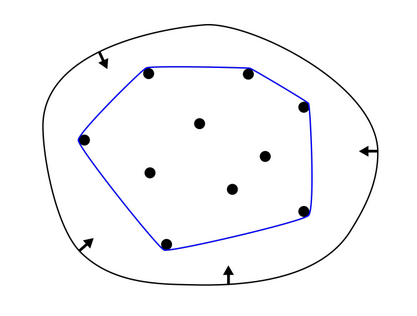
\includegraphics[scale = 0.4]{pix/convex_hull.png}
\end{figure}

\textbf{Алгоритм Джарвиса.} 
\begin{enumerate}
    \item Пусть $P_0$ — самая левая (из них самая нижняя) точка.
    \item Введем $P_1$ — точка с минимальным углом относительно между осью $OY$ и $P_0P_1$.
    \item $\forall i > 1$ точка $P_i$ определяется как точка с максимальным углом $\angle P_{i-2}P_{i-1}P_i$
\end{enumerate}

\begin{figure}[h]
    \centering
    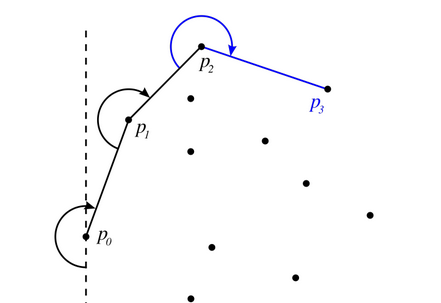
\includegraphics[scale = 0.8]{pix/convex_hull_Jarvis.png}
\end{figure}

\textbf{Aсимптотика:} Поиск $P_0$, $P_1$ занимает $\mathcal{O}(n)$ времени, так как это наивный перебор. Поиск $P_i$ составит в свою очередь аналогично $\mathcal{O}(n)$, так как надо перебрать все точки. Пусть $h$ — число точек в выпуклой оболочке, тогда время работы составит $\Theta(nh) = \mathcal{O}(n^2)$.

\pagebreak

\section{49. Выпуклая оболочка. Алгоритм Грехема.}
\textbf{Алгоритм Грехема.} 
\begin{enumerate}
    \item Пусть $P_0$ — самая нижняя (из них самая левая) точка.
    \item Отсортируем точки относительно угла между $OX$ и $P_0P_i$ (при равенстве по |$P_0P_i$|).
    \item Добавим в стек $S$ точки $P_0, P_1$.
    \item Если угол поворота(против часовой стрелки) от $S.prevtop() S.top()$ до $S.top()P_i$ меньше $\pi$, добавляем $P_i$ в стек. Иначе, пока угол больше $\pi$, извлекаем из стека последнюю точку.
\end{enumerate}
В конце алгоритма в стеке будет лежать выпуклая оболочка.\newline

%\begin{figure}[h]
%    \centering
%    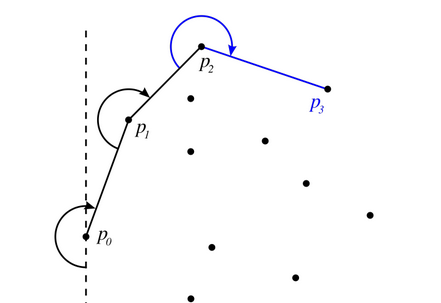
\includegraphics[scale = 0.8]{pix/convex_hull_Jarvis.png}
%\end{figure}

\textbf{Aсимптотика:} Первые две стадии: поиск $P_0$ и сортировка работают за $O(n\cdot\log n)$
времени. За сколько работает проход стеком? За линейное время, так как каждая точка попадает в стек ровно раз и не более одного раза оттуда удаляется.

Таким образом, суммарное время работы составит $O(n\cdot\log n)$.\newline

Псевдокод:
\begin{lstlisting}
p0 = TheLeftestAmongTheLowests(points);
sort(points, by_polar_from(p0));
stack<point> s;
s.push(points[0]), s.push(points[1]);
for (int i = 2; i < points.size(); ++i) {
  while (s.size() >= 2 &&
      Angle(s.prevtop(), s.top(), points[i]) < pi) {
        s.pop();
  }
  s.push(points[i]);
}
\end{lstlisting}
\pagebreak

\section{50. Сумма Минковского. Выпуклость суммы Минковского для двух выпуклых фигур. Алгоритм
построения для двух выпуклых многоугольников за линейное время (корректность б/д).}
\Def Пусть $A, B$ — множества элементов линейного пространства $L$, тогда суммой Минковского назовем $A \oplus B = \{a + b \ |\  a \in A, \ b \in B\}$.

Далее будем рассматривать в качестве $L$ плоскость или, так
называемое, $\R^2$. Под $a$ и $b$ подразумеваются радиус вектора этих точек.\newline

\Statement Сумма Минковского двух выпуклых фигур выпукла.

\Proof Рассмотрим произвольные $A_1$, $A_2 \in A$, тогда $\forall t \in [0, 1] A_t = A_1 + (A_2 - A_1)t \in A$.\newline
Аналогично $\forall t \in [0, 1] B_t = B_1 + (B_2 - B_1)t \in B$. \newline
$A_t + B_t = (A_1 + B_1) + ((A_2 + B_2) - (A_1 + B_1))t \in A \oplus B$ и это верно для произвольного $t \in [0, 1]$.\newline

\Statement Если $S, T$ - выпуклые многоугольники, то $S \oplus T$ - выпуклый многоугольник.

\Statement Если $S = \{S_1, \dots, S_n\}$ и $T = \{T_1, \dots, T_m\}$ - выпуклые многоугольники, то \begin{enumerate}
    \item В $S \oplus T$ $\mathcal{O}(n+m)$ сторон
    \item $S \oplus T = conv(\{ S_i + T_j \ | \ i \in [1, n], j\in [1, m]\})$
\end{enumerate}

\Proof Рассмотрим вектор $d \in \R^2$. Рассмотрим семейство прямых Р, для которых $d$ является нормалью. Тогда крайней точкой многоугольника в направлении $d$ назовем такую вершину $А$, что если через нее провести прямую из Р, то весь многоугольник окажется в одной полуплоскости.

Заметим, что если рассмотреть крайние вершины $S$ и $T$ в направлении $d$, то их сумма окажется тоже крайней вершиной $S \oplus T$ в данном направлении. Действительно, рассмотрим две точки, суммой которых она является. Рассмотри проекции их радиус-векторов на $d$. Тогда при взятии точек с наибольшими проекциями на $d$ мы должны были получить крайнюю точку.

Тогда можно заметить, что если рассмотреть $d$ такой, что он ортогонален одной из сторон $S$, тогда
данная сторона будет состоять из крайних точек в направлении $d$, а значит и данная сторона будет крайней в $S \oplus T$.
Из наблюдения выше рассмотрим вектора, ортогональные каждой из $|S| + |T|$ сторон, тогда они будут крайними в $S \oplus T$, откуда следует, что в $S \oplus T$ будет не больше $|S| + |T|$ вершин. Более того, выпуклость вытекает из построения того, что стороны были крайними.

Из последнего пункта последнего утверждения можно получить \textbf{наивный алгоритм} нахождения суммы Минковского:
\begin{enumerate}
    \item Пусть $C_{ij} = A_i + B_j$
    \item Построим выпуклую оболочку на $\{C_{ij}\}_{i,j=1} ^ {|A||B|}$
\end{enumerate}
\textbf{Асимптотика:} $\mathcal{O}(n^2 \cdot \log n)$, поскольку это время работы алгоритма, строящего выпуклую оболочку на $n^2$ точках.\newline

\textbf{Оптимальный алгоритм:}
\begin{enumerate}
    \item Пусть $A_0$ и $B_0$ — самые нижние (из них самые левые) точки $A$ и $B$ соответственно, $C_0 = A_0 + B_0$.
    \item Сделаем циклический сдвиг $A$ и $B$ так, чтобы обход был против часовой стрелки и начинался с соответственно $A_0$ и $B_0$.
    \item Пусть $\text{v}^A_i = \overline{A_{i - 1}A_i}, \ \text{v}^B_i = \overline{B_{i-1}B_i}$. Заметим, что массивы $\text{v}^A$ и $\text{v}^B$ отсортированы по полярному углу.
    \item Построим $\text{v}^C = Merge(\text{v}^A, \text{v}^B)$.
    \item Последовательно откладываем от $C_0$ вектора из массива $\text{v}^C$ , то есть $C_i = C_{i-1} + v^C_i$.
\end{enumerate}
Полученный набор $C_i$ -- искомый многоугольник.

\textbf{Асимптотика:} \begin{enumerate}
    \item Построение $C_0$ и препроцессинг многоугольников выполняется за $\mathcal{O}(|A| + |B|)$.
    \item Построение  $\text{v}^A$, $\text{v}^B$ выполняется за $\mathcal{O}(|A| + |B|)$.
    \item Слияние  $\text{v}^A$, $\text{v}^B$ выполняется за $\mathcal{O}(|A| + |B|)$.
    \item Построение  $C_i$ выполняется за $\mathcal{O}(|A| + |B|)$.
\end{enumerate}
Итоговое время работы: $\mathcal{O}(|A| + |B|)$.

\pagebreak

\section{51. Поиск пары самых удаленных точек на плоскости за $O(N log N)$.}
\Def Диаметром $S \subset \R^2, |S| < \infty$ называют такую пару $a, b \in S$, на которой достигается максимум $||a - b||$.

\Task Надо найти диаметр по евклидовой метрике.

\Statement Концами диаметра являются две вершины выпуклой оболочки $S$.

\Proof Пусть $AB$ — диаметр $S$, при этом $B$ — не вершина выпуклой оболочки. Рассмотрим луч $AB$ и пересечем его с $conv(S)$ в точке $C$. Тогда $|AC| \Ge |AB|$. Теперь пусть $PQ$ — сторона $conv(S)$, по которой луч $AB$ пересек $conv(S)$. Очевидно, $\max(|AP|, |AQ|) > |AC| \Ge |AB|$, откуда $AB$ не диаметр.

\begin{figure}[h]
    \centering
    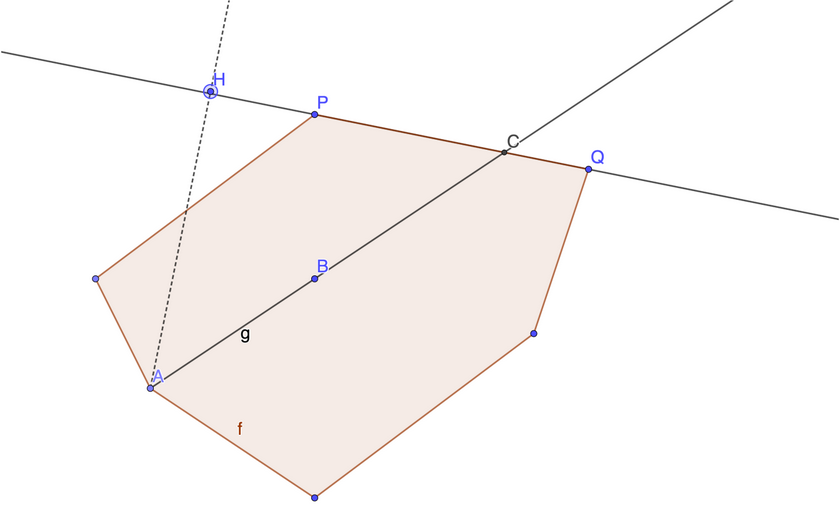
\includegraphics[scale = 0.8]{pix/pair_far1.png}
\end{figure}

\Task Дан выпуклый многоугольник $P_0, \dots, P_{n-1}$. Найдите пару $i, j \in \overline{(0, n - 1)}$, что $||P_i - P_j ||$ по евклидовой метрике максимально.

\vspace{\baselineskip}

\Def Прямая $L$ опорная для выпуклого многоугольника $P_0, \dots, P_{n-1}$, если вся внутренность лежит по одну полуплоскость относительно $L$ и $\exists i : P_i \in L$.

\Statement Пусть $L_1$ и $L_2$ — две параллельные опорные прямые фигуры Ф, расстояние между которыми имеет максимальное значение. $A_1$ и $A_2$ — граничные точки фигуры Ф, принадлежащие соответственно прямым $L_1$ и $L_2$. Тогда отрезок $A_1A_2$ перпендикулярен обеим прямым $L_1$ и $L_2$.

\Proof Предположим, что это не так. Тогда расстояние между прямыми $L_1$ и $L_2$ было бы меньше, чем отрезок $A_1A_2$, и тем более меньше, чем расстояние между двумя опорными прямыми $L^{'}_{1}$ и $L^{'}_{2}$ фигуры Ф, перпендикулярными к отрезку $A_1A_2$, что противоречит условию.


(рисунок ниже)

\begin{figure}[h]
    \centering
    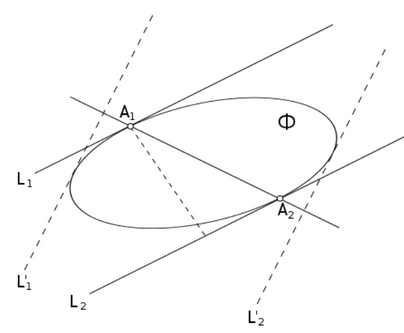
\includegraphics[scale = 1]{pix/pair_far3.png}
\end{figure}

\vspace{\baselineskip}

\Th\textit{(о диаметре)} Диаметр выпуклого многоугольника равен максимальному расстоянию между параллельными опорными прямыми.

\Proof Пусть $L_1$ и $L_2$ — параллельные опорные прямые, на которых достигается максимальное расстояние $d$. Тогда $A_1A_2 \perp L_i$. Допустим, что есть две точки $B_1, B_2$, расстояние между которыми больше. Тогда рассмотрим ортогональные $B_1B_2$ опорные прямые $L^{'}_{1}, L^{'}_{2}$. $|B_1B_2| \Le dist(L^{'}_{1}, L^{'}_{2}) \Le d$.

\vspace{\baselineskip}

\Alg
\begin{enumerate}
    \item Построим $P = conv(S)$.
    \item Пусть $A_1 = P_0$, тогда $A_2$ — максимально удаленная от $A_1$ точка $P$.
    \item Заведем два указателя на $A_1$ и $A_2$ и будем идти против часовой стрелки. Двигается тот указатель, который указывает на угол меньший до проворота.
\end{enumerate}

\begin{figure}[h]
    \centering
    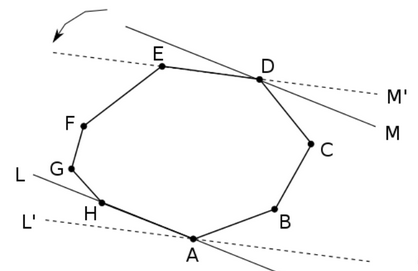
\includegraphics[scale = 1]{pix/pair_far2.png}
\end{figure}
\pagebreak

\section{52. Поиск пары ближайших точек на плоскости за $O(N log N)$.}
\Alg

\begin{enumerate}
    \item Отсортируем все точки по абсциссе.
    \item Разделим медианой по абсциссе точки на две группы.
    \item Найдем в каждой рекурсивно ответ.
    \item Сольем две половины и найдем оптимальный ответ.
\end{enumerate}

Пусть $d\,=\,min(d_1,\,d_2)$, где $d_1$ — ответ от левой половины, а $d_2$ — от правой.
Ответ может быть либо равен d, либо надо рассмотреть пары точек из обеих частей.
Заметим, что если мы разбили по $x_0$ пополам, то надо рассматривать только точки с абсциссой в пределах $[x_0\,-\,d,\,x_0\,+\,d]$

Пусть $P_i$ попадает в полосу, обозначим за $C(P_i)$ прямоугольник по
абсциссе в $[x_0\,-\,d,\,x_0\,+\,d]$, а по ординате $[P_i.y,\,P_i.y\,+\,d]$.\\
Разобьем $C(P_i)$ на 8 квадратов $\frac{d}{2} \times \frac{d}{2}$. Не может быть двух точек в одном из квадратов, так как иначе расстояние на одной из половин было бы меньше $d$.

\drawsomesmall{pix/search_a_pair_of_nearby_points.png}

Откуда для каждой точки в полосе $O(1)$ точек кандидатов.\\
Отсортируем точки по ординате и будем идти двумя указателями по
тем что в полосе, ища минимальное расстояние.

\subsection*{Асимптотика}

Заметим, что если время слияния двух мнодеств по n точек равно $Merge(n)$, то итоговое время работы: $T(n)\,=\,2T(n/2)\,+\,Merge(n)$.\\
По мастер-теореме $T(n)\,=\,O(Merge(n)\, \cdot \,log\,n)$.\\
В слиянии сначала происходит сортировка, а потом два указателя, по
$O(1)$ времени на каждое положение, а значит $Merge(n)\,=\,O(n\,log\,n)$.\\
То есть время работы равно $O(n\,log^2\,n)$.

\Note Если алгоритм переупорядочивает набор точек, уже отсортированных
по y, то вместо того, чтобы заново сортировать набор на стадии слияния применим Merge за линейное время!
Тогда $Merge(n)\,=\,O(n)$ и итоговое время работы равно $O(n\,log\,n)$.

\pagebreak
